\documentclass[11pt,a4paper]{article}

\usepackage[T1]{fontenc}
\usepackage[utf8]{inputenc}
\usepackage{lmodern}
\usepackage[a4paper,margin=0.95in,top=0.95in,bottom=1.0in]{geometry}
\usepackage{microtype}
\usepackage{setspace}
\usepackage{amsmath,amssymb}
\usepackage{booktabs,tabularx,array,longtable,multirow}
\usepackage{graphicx}
\usepackage{xcolor}
\usepackage{float}
\usepackage{caption}
\usepackage{subcaption}
\usepackage{enumitem}
\usepackage{hyperref}
\usepackage{fancyhdr}
\usepackage{tikz}
\usetikzlibrary{arrows.meta,positioning,calc,fit,shapes.geometric,shapes.misc,backgrounds}
\usepackage{siunitx}

\graphicspath{
  {../plots/}
  {../plots/extended_research/}
  {../plots/lifetime_modeling/}
  {../../results/cross_dataset_research/plots/}
  {../../results/vmd/}
  {../../results/modeling/}
  {../../results/interpretation/}
  {../../results/feature_selection/}
  {../../results/eda/}
}

\hypersetup{
  colorlinks=true,
  linkcolor=teal!55!black,
  urlcolor=blue!55!black,
  citecolor=teal!55!black,
  pdftitle={From Sensor Signatures to Survival Curves},
  pdfauthor={Amrit Lahari, Sukrit Agarwal, Pushkar Agrawal, Amit Kumar Jain},
  pdfsubject={Physics-regularized tool wear and tool-life modeling}
}

\setstretch{1.06}
\setlength{\parindent}{0pt}
\setlength{\parskip}{0.35em}
\setlist[itemize]{leftmargin=1.4em,itemsep=0.18em,topsep=0.18em}
\setlist[enumerate]{leftmargin=1.6em,itemsep=0.18em,topsep=0.18em}
\setlength{\headheight}{13pt}
\pagestyle{fancy}
\fancyhf{}
\lhead{From Sensor Signatures to Survival Curves}
\rhead{\thepage}

% --- float placement tuning to reduce empty space on pages ---
\renewcommand{\topfraction}{0.95}
\renewcommand{\bottomfraction}{0.90}
\renewcommand{\textfraction}{0.05}
\renewcommand{\floatpagefraction}{0.92}
\renewcommand{\dbltopfraction}{0.95}
\renewcommand{\dblfloatpagefraction}{0.92}
\setcounter{topnumber}{4}
\setcounter{bottomnumber}{3}
\setcounter{totalnumber}{6}
\setcounter{dbltopnumber}{4}
\setlength{\textfloatsep}{8pt plus 2pt minus 2pt}
\setlength{\floatsep}{6pt plus 2pt minus 2pt}
\setlength{\intextsep}{8pt plus 2pt minus 2pt}
\setlength{\dbltextfloatsep}{8pt plus 2pt minus 2pt}
\setlength{\abovecaptionskip}{4pt}
\setlength{\belowcaptionskip}{2pt}
\captionsetup{font=small,labelfont=bf,skip=4pt}
\flushbottom

\definecolor{ink}{HTML}{172026}
\definecolor{muted}{HTML}{5C6A73}
\definecolor{teal}{HTML}{147C7C}
\definecolor{amber}{HTML}{C67C18}
\definecolor{brick}{HTML}{A64032}
\definecolor{green}{HTML}{2D7A46}
\definecolor{panel}{HTML}{F4F7F8}
\definecolor{linegray}{HTML}{CBD5DA}

\newcommand{\vb}{V\!B}
\newcommand{\vbtr}{V\!B_{\mathrm{tr}}}
\newcommand{\vbf}{V\!B_{\mathrm{f}}}
\newcommand{\ttr}{t_{\mathrm{tr}}}
\newcommand{\phii}{\phi}
\newcommand{\earlyexp}{m_{\mathrm{e}}}
\newcommand{\lateexp}{m_{\mathrm{l}}}
\newcommand{\code}[1]{\texttt{#1}}
\newcommand{\dataset}[1]{\textsf{#1}}
\newcommand{\figref}[1]{Figure~\ref{#1}}
\newcommand{\tabref}[1]{Table~\ref{#1}}
\newcommand{\eqnref}[1]{Equation~\eqref{#1}}
\newcommand{\smallcaps}[1]{\textsc{#1}}
\newcommand{\modelname}{\smallcaps{PREDICT}}

\newcolumntype{Y}{>{\raggedright\arraybackslash}X}
\newcolumntype{R}{>{\raggedleft\arraybackslash}p{1.35cm}}

\title{\bfseries From Sensor Signatures to Survival Curves\\[0.25em]
  \large\itshape A Physics-Regularized Digital Twin for Milling Tool Wear and Tool-Life Forecasting}
\author{%
  \large Amrit Lahari \quad Sukrit Agarwal \quad Pushkar Agrawal \\[0.4em]
  \normalsize\itshape Supervised by\ \ \large\bfseries Dr.~Amit Kumar Jain}
\date{May 2026}

\begin{document}

% =====================================================================
%  SOP COVER PAGE
% =====================================================================
\begin{titlepage}
  \thispagestyle{empty}
  \centering
  \vspace*{0.5cm}
  {\Large\bfseries Study Oriented Project (SOP) Report\par}
  \vspace{1.4cm}
  {\Large\itshape ``From Sensor Signatures to Survival Curves:\\[0.25em]
  A Physics-Regularized Digital Twin for Milling Tool\\[0.15em]
  Wear and Tool-Life Forecasting''\par}
  \vspace{1.4cm}

  {\large\bfseries Submitted by\par}
  \vspace{0.45cm}
  \renewcommand{\arraystretch}{1.35}
  \begin{tabular}{|c|p{4.4cm}|p{3.3cm}|p{5.4cm}|}
    \hline
    \textbf{S.No.} & \textbf{Full Name} & \textbf{Student ID} & \textbf{Official Email} \\
    \hline
    1 & Amrit Lahari    & 2023A4PS0442P & f20230442@pilani.bits-pilani.ac.in \\
    \hline
    2 & Sukrit Agarwal  & 2023A4PS0431P & f2023043@pilani.bits-pilani.ac.in \\
    \hline
    3 & Pushkar Agrawal & 2023A4PS0425P & f20230425@pilani.bits-pilani.ac.in \\
    \hline
  \end{tabular}
  \renewcommand{\arraystretch}{1.0}

  \vspace{1.0cm}
  \begin{tabular}{|p{4.0cm}|p{4.4cm}|p{3.0cm}|p{3.0cm}|}
    \hline
    \textbf{Semester \& Year} & \textbf{Program and Department} & \textbf{Project Start Date} & \textbf{Project End Date} \\
    \hline
    2nd Semester; 3rd Year & B.E.~Mechanical Engineering, Department of Mechanical Engineering & 06/January/2026 & 01/May/2026 \\
    \hline
  \end{tabular}

  \vspace{1.0cm}
  {\large\bfseries Supervisor\par}
  \vspace{0.25cm}
  {\large Dr.~Amit Kumar Jain\par}
  {\small\itshape Department of Mechanical Engineering\par}

  \vfill
  {\large\bfseries Birla Institute of Technology and Science, Pilani\par}
  \vspace{0.45cm}
  {\large 01 / May / 2026\par}
\end{titlepage}

% =====================================================================
%  RESEARCH PAPER (Elsevier-style title block)
% =====================================================================
\maketitle
\thispagestyle{empty}

\begin{abstract}\noindent
We study \textbf{milling tool wear}, \textbf{tool-health failure detection}, and \textbf{threshold-crossing tool-life estimation} using three complementary public datasets: \dataset{NUAA}/\dataset{UniWear} orthogonal milling experiments, \dataset{PHM2010} cutter wear traces, and the \dataset{NASA} milling run-to-failure records. The objective is \emph{not only} to reduce pointwise wear error, but to build an interpretable, simulator-ready model that explains load effects, supports uncertainty bands, and connects signal-processing evidence to practical tool replacement. We propose a \textbf{physics-regularized piecewise wear law}: a sub-linear early regime with exponent \(\earlyexp=\mathbf{0.64}\) (verified on NUAA and PHM2010) and an accelerated late regime with exponent \(\lateexp=\mathbf{1.29}\) (extracted from NASA). A reference-point process-load function \(\phi(n,f_z,a_p)\) is fitted from NUAA, with \emph{feed emerging as the strongest driver}. We then train multiple wear regressors, invert them to threshold-crossing life estimates, and compare against censored accelerated-failure-time (AFT) equations. The best wear regressor (\textbf{Gradient Boosting}) does \emph{not} produce the best event-life forecast after inversion --- \textbf{optimizing wear RMSE is not equivalent to optimizing threshold-crossing life}. Frequency-domain evidence from \textbf{variational mode decomposition (VMD)} raises the strongest absolute correlation with wear from \(0.4806\) to \(\mathbf{0.5607}\). Bootstrap intervals, residual diagnostics, and early-window calibration tests describe where the model is stable and where it is under-identified. The result is a research-grade digital-twin prototype useful for scenario ranking and explanation, but requiring broader ingestion of newer full-life milling datasets before industrial deployment.

\medskip
\noindent\textbf{Keywords:}\ tool wear, tool-life forecasting, physics-regularized regression, variational mode decomposition, accelerated failure time, digital twin.
\end{abstract}

\section{Introduction}

\subsection{Problem}

Milling tool wear is not a single regression problem. A tool can spend long periods in a slow early-wear regime, then enter an accelerated damage regime where a small amount of additional cutting time produces a large increase in flank wear. Datasets emphasize different parts of this story. Some datasets capture many process settings but short or synthetic lives. Others contain full run-to-failure trajectories but few cutting conditions. A useful research model therefore has to answer four questions at once:

\begin{enumerate}
  \item What wear curve explains the physical progression from early wear to accelerated wear?
  \item How do spindle speed, feed, and depth alter the rate of that curve?
  \item Which sensor signatures provide evidence that the tool is moving toward a failure threshold?
  \item Can a model trained on wear observations be inverted into a practical lifetime equation?
\end{enumerate}

The local repository addresses these questions with a staged approach. The first stage extracts signal features and cross-dataset baselines. The second stage builds a piecewise wear equation. The third stage extends the equation with uncertainty and residual diagnostics. The fourth stage explicitly trains wear models, inverts them into lifetime predictions, and compares them with survival-style accelerated-failure-time models.

\subsection{Main Contributions}

\begin{itemize}
  \item \textbf{A dataset-role framework} that uses NUAA for load-dependent early wear, PHM2010 for early-exponent transfer, and NASA for accelerated late-stage behavior.
  \item \textbf{A compact piecewise wear model} with interpretable exponents and a process-load intensity function.
  \item \textbf{A cross-dataset health pipeline} that evaluates wear regression and failure classification under grouped validation.
  \item \textbf{VMD-based frequency evidence} showing that decomposed vibration, acoustic-emission, and spindle-current signatures improve the strongest absolute correlation with wear from \(0.4806\) to \(\mathbf{0.5607}\).
  \item \textbf{A lifetime-model extraction pipeline} that trains multiple wear models, inverts them into threshold-crossing estimates, and exposes the mismatch between wear RMSE and life accuracy.
  \item \textbf{Censored accelerated-failure-time equations} for NUAA and material-aware NASA life behavior.
  \item \textbf{Bootstrap uncertainty, residual diagnostics, and calibration tests} that describe where the current model is stable and where it remains under-identified.
\end{itemize}

\begin{figure}[!htbp]
  \centering
  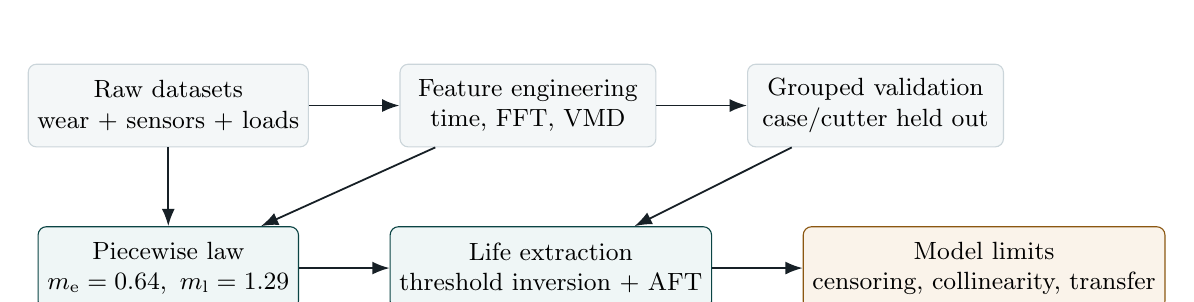
\begin{tikzpicture}[node distance=1.0cm and 1.15cm]
    \tikzset{
      block/.style={rounded corners=3pt,draw=linegray,fill=panel,minimum width=3.25cm,minimum height=1.05cm,align=center,font=\small},
      result/.style={rounded corners=3pt,draw=teal!55!black,fill=teal!7,minimum width=3.25cm,minimum height=1.05cm,align=center,font=\small},
      warn/.style={rounded corners=3pt,draw=amber!70!black,fill=amber!9,minimum width=3.25cm,minimum height=1.05cm,align=center,font=\small},
      arrow/.style={-{Latex[length=2.2mm]},draw=ink,line width=0.65pt}
    }
    \node[block] (raw) {Raw datasets\\wear + sensors + loads};
    \node[block,right=of raw] (feat) {Feature engineering\\time, FFT, VMD};
    \node[block,right=of feat] (cv) {Grouped validation\\case/cutter held out};
    \node[result,below=of raw] (law) {Piecewise law\\\(\earlyexp=0.64,\ \lateexp=1.29\)};
    \node[result,right=of law] (life) {Life extraction\\threshold inversion + AFT};
    \node[warn,right=of life] (limits) {Model limits\\censoring, collinearity, transfer};
    \draw[arrow] (raw) -- (feat);
    \draw[arrow] (feat) -- (cv);
    \draw[arrow] (raw) -- (law);
    \draw[arrow] (feat) -- (law);
    \draw[arrow] (law) -- (life);
    \draw[arrow] (cv) -- (life);
    \draw[arrow] (life) -- (limits);
  \end{tikzpicture}
  \caption{Research architecture followed in the repository. The workflow separates signal evidence, physics-regularized equation building, grouped validation, and survival-aware life estimation.}
  \label{fig:research-architecture}
\end{figure}

\section{Literature Review}

\subsection{Why Biology and Survival Modeling Matter}

The lifetime rework borrowed ideas from survival analysis, including accelerated-failure-time modeling and censoring. This is common outside machining, especially in medicine and biology, where time-to-event data are often censored because patients leave a study or an event has not occurred by the observation cutoff. Tool-life data have the same structure: a tool may not reach the failure threshold before the experiment ends. Treating those runs as ordinary non-events wastes information and biases the model.

Deep survival models, Gaussian-process remaining-useful-life methods, physics-informed Gaussian processes, and physics-informed neural networks are useful pivots from adjacent domains. The repository does not blindly import these methods. Instead, it uses their modeling idea: preserve censoring, quantify uncertainty, and embed physical constraints where the data are too sparse to identify a purely black-box model.

\subsection{Literature Positioning}

\begin{longtable}{p{3.0cm}p{4.0cm}p{6.7cm}}
  \caption{External literature themes and how they influence this project.}
  \label{tab:literature-themes}\\
  \toprule
  Theme & Representative source type & Influence on this research \\
  \midrule
  \endfirsthead
  \toprule
  Theme & Representative source type & Influence on this research \\
  \midrule
  \endhead
  PHM milling benchmarks & PHM competition and benchmark reviews & Motivates grouped validation, run-level splits, and caution about leakage across adjacent samples. \\
  Public full-life milling datasets & 2025 \emph{Scientific Data} milling datasets & Identifies next ingestion targets for broader validation beyond the three local datasets. \\
  Survival analysis & DeepSurv and accelerated-failure-time literature & Provides a principled vocabulary for event labels, right censoring, and life prediction under incomplete runs. \\
  RUL uncertainty & PHM RUL uncertainty and Gaussian-process RUL work & Motivates prediction intervals and coefficient bootstrap rather than single deterministic life numbers. \\
  Physics-informed learning & PINNs, physics-informed GP, and PI-KAF tool-wear monitoring & Supports the project choice to combine a mechanistic wear equation with statistical features and ML models. \\
  Frequency decomposition & VMD and modal signal-processing literature & Supports modal features as interpretable signal evidence for wear progression. \\
  \bottomrule
\end{longtable}

\subsection{Research Gaps}

Synthesizing the literature against the available milling datasets exposes four gaps that motivate this work:

\begin{enumerate}
  \item \textbf{Dataset role mixing.} Most prior tool-wear studies pool heterogeneous datasets into a single regression, ignoring that some datasets (e.g.\ \dataset{NUAA}) sample many process conditions but truncate before failure, while others (e.g.\ \dataset{NASA}) follow tools to severe wear under a narrower design. Pooling without role separation conflates early and late wear physics.
  \item \textbf{Missing piecewise physics priors.} Single-exponent power-law fits compromise between the slow early regime and the accelerated late regime, smoothing over the transition that matters most for replacement decisions.
  \item \textbf{Wear-RMSE bias in life prediction.} Existing benchmarks rank models by pointwise wear error and assume the same ranking carries over to lifetime forecasting. The threshold-inversion step that converts wear models into life estimates is rarely tested under censoring.
  \item \textbf{Sparse uncertainty quantification.} Bootstrap intervals, calibration tests, and survival-aware lifetime intervals are often missing from machining-monitoring papers, leaving deterministic single-number predictions that are poorly suited to industrial decision support.
\end{enumerate}

This work addresses all four gaps directly: a dataset-role framework, a piecewise wear law with regime-specific exponents, an inversion-aware lifetime evaluation, and bootstrap-based uncertainty propagation.

\section{Methodology}

\subsection{Data Sources and Evidence Roles}

\subsubsection{Dataset Inventory}

The repository contains or references three primary milling sources. They are not interchangeable, so the research assigns each dataset a specific inferential role. This is preferable to pooling everything into one opaque regression table, because the datasets differ in time base, sensors, process variables, material, failure threshold, and whether the experiment reaches severe wear.

\begin{table}[!htbp]
  \centering
  \caption{Primary datasets and their research roles.}
  \label{tab:dataset-roles}
  \small
  \begin{tabularx}{\textwidth}{p{2.3cm}p{2.9cm}p{2.4cm}Y}
    \toprule
    Dataset & Local role & Main measurements & Why it matters \\
    \midrule
    NUAA / UniWear & Early wear and process-condition law & Wear, spindle speed, feed per tooth, axial depth & Supplies process variation needed to fit a load-intensity function and lifetime surfaces. It includes censored runs, which makes survival-aware modeling necessary. \\
    PHM2010 & Early-regime transfer check & Cutter wear traces and derived features & Tests whether the early exponent learned from NUAA is a local artifact or a transferable early-wear slope. \\
    NASA Milling & Late-stage acceleration and material behavior & Vibration, acoustic emission, spindle current, wear, feed, depth, material & Contains severe wear progression and rich sensors, making it the best local source for accelerated wear, frequency-domain evidence, and material-aware survival behavior. \\
    \bottomrule
  \end{tabularx}
\end{table}

\subsubsection{Data Role Diagram}

\begin{figure}[!htbp]
  \centering
  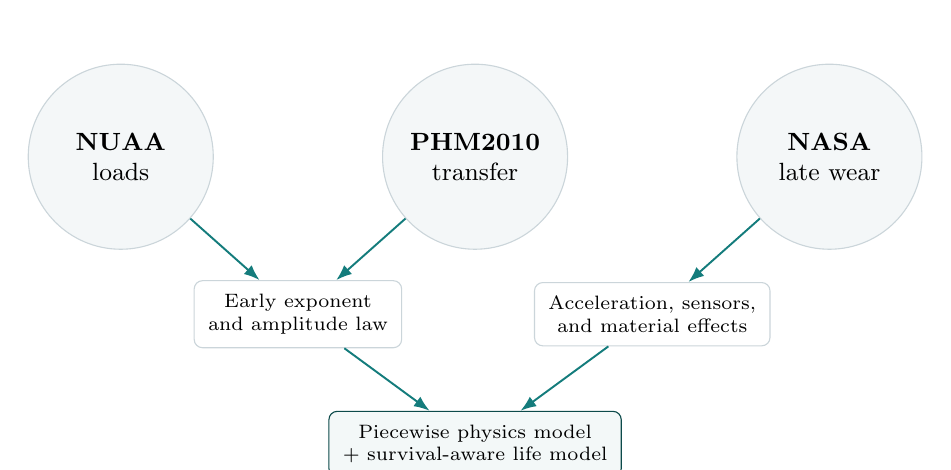
\begin{tikzpicture}
    \tikzset{
      ds/.style={circle,draw=linegray,fill=panel,minimum size=2.35cm,align=center,font=\small},
      callout/.style={rounded corners=3pt,draw=linegray,fill=white,align=center,font=\scriptsize,inner sep=5pt},
      arrow/.style={-{Latex[length=2mm]},draw=teal,line width=0.7pt}
    }
    \node[ds] (nuaa) at (0,0) {\textbf{NUAA}\\loads};
    \node[ds] (phm) at (4.5,0) {\textbf{PHM2010}\\transfer};
    \node[ds] (nasa) at (9,0) {\textbf{NASA}\\late wear};
    \node[callout] (early) at (2.25,-2.0) {Early exponent\\and amplitude law};
    \node[callout] (late) at (6.75,-2.0) {Acceleration, sensors,\\and material effects};
    \node[callout,draw=teal!60!black,fill=teal!5] (model) at (4.5,-3.65) {Piecewise physics model\\+ survival-aware life model};
    \draw[arrow] (nuaa) -- (early);
    \draw[arrow] (phm) -- (early);
    \draw[arrow] (nasa) -- (late);
    \draw[arrow] (early) -- (model);
    \draw[arrow] (late) -- (model);
  \end{tikzpicture}
  \caption{The datasets act like complementary evidence sources. NUAA and PHM2010 constrain the early regime, while NASA constrains late acceleration and sensor signatures.}
  \label{fig:dataset-role-diagram}
\end{figure}

\subsubsection{Failure Thresholds}

The failure classification task uses dataset-specific thresholds because the measurement scale and experimental intent differ. The thresholds are not presented as universal industrial replacement limits; they are operational labels used to compare health markers within each dataset.

\begin{table}[!htbp]
  \centering
  \caption{Dataset-specific tool-health failure labels used in the cross-dataset research pipeline.}
  \label{tab:failure-thresholds}
  \small
  \begin{tabular}{lrrr}
    \toprule
    Dataset & Samples & Threshold & Failure rate \\
    \midrule
    PHM2010 & 945 & \(0.150~\mathrm{mm}\) & 0.1725 \\
    NASA & 146 & \(0.300~\mathrm{mm}\) & 0.4795 \\
    UniWear & 649 & \(0.220~\mathrm{mm}\) & 0.2743 \\
    \bottomrule
  \end{tabular}
\end{table}

\begin{figure}[!htbp]
  \centering
  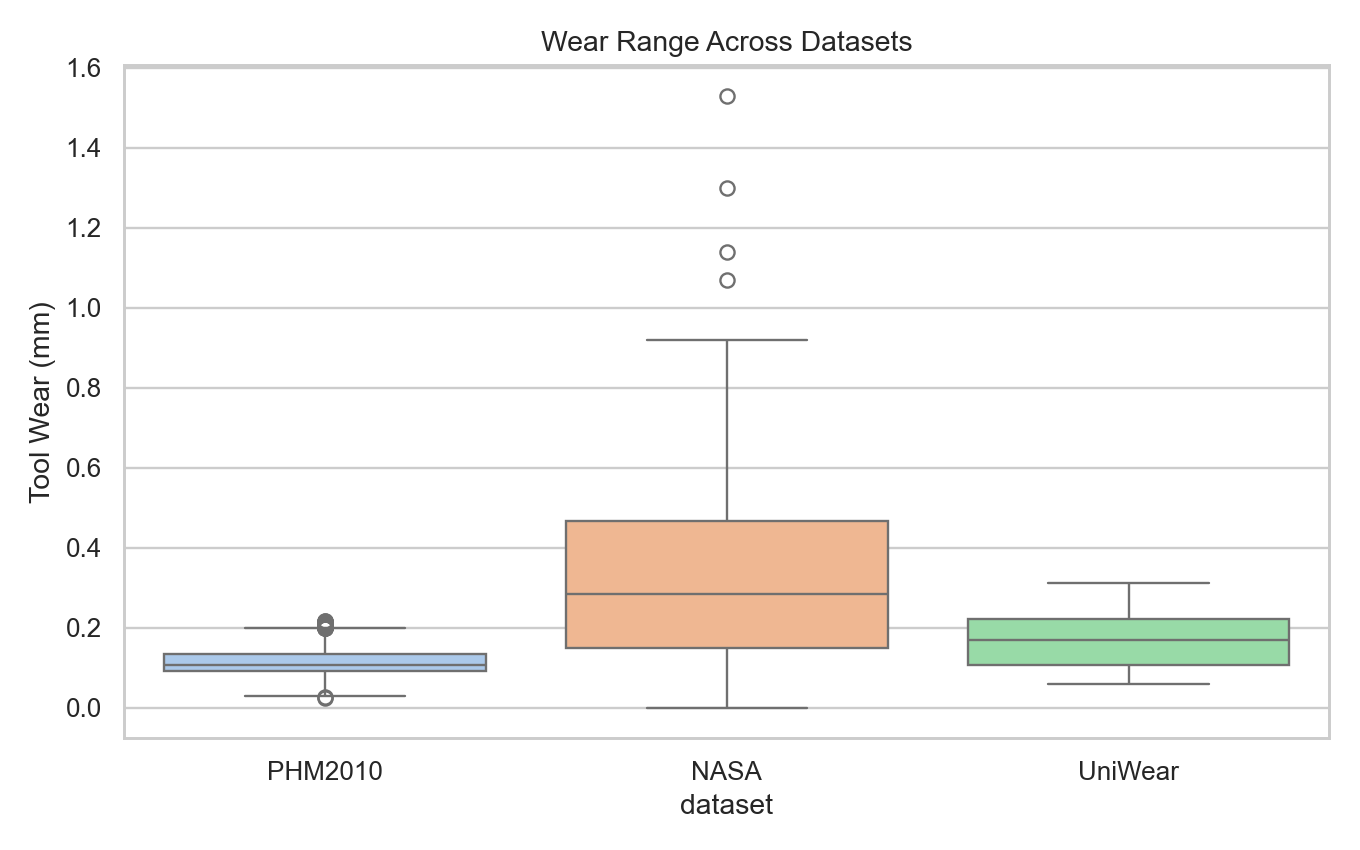
\includegraphics[width=0.85\textwidth]{dataset_wear_distribution.png}
  \caption{Wear distributions across local datasets. The different ranges motivate dataset-specific thresholds and role-specific modeling rather than direct pooling.}
  \label{fig:wear-distribution}
\end{figure}

\subsection{Feature Engineering and Frequency Evidence}

\subsubsection{Feature Families}

The repository extracts compact signal features from time-domain and frequency-domain measurements. The shared feature vocabulary includes mean, standard deviation, root-mean-square, absolute mean, peak-to-peak range, skew-like statistics, kurtosis-like statistics, crest factor, quantiles, FFT energy, dominant FFT bin, FFT centroid, and spectral entropy. The NASA pipeline also includes VMD features computed over vibration, acoustic-emission, spindle-current AC, and spindle-current DC channels.

\begin{table}[!htbp]
  \centering
  \caption{Feature families and interpretation.}
  \label{tab:feature-families}
  \small
  \begin{tabularx}{\textwidth}{p{2.7cm}p{4.0cm}Y}
    \toprule
    Family & Examples & Tool-wear interpretation \\
    \midrule
    Time-domain level & mean, RMS, absolute mean & Captures load and energy growth as cutting becomes less efficient. \\
    Time-domain shape & skewness, kurtosis, crest factor, quantiles & Captures impulsive events, chatter bursts, rubbing, and intermittent edge damage. \\
    Frequency-domain energy & FFT energy, FFT peak, centroid, entropy & Captures shifts in vibration and acoustic-emission structure as wear changes cutting dynamics. \\
    VMD mode features & mode energy, entropy, center frequency, mode kurtosis & Separates mixed sensor signals into interpretable bands, improving some wear correlations over raw features. \\
    Process variables & speed, feed, axial depth, material & Anchor the statistical model in machining physics and enable scenario simulation. \\
    \bottomrule
  \end{tabularx}
\end{table}

\subsubsection{Variational Mode Decomposition}

The VMD pass decomposes NASA signals into \(K=5\) modes with \(\alpha=2000\) and \(\tau=0\). It produces \textbf{390 VMD features} over sensors \code{vib\_spindle}, \code{vib\_table}, \code{AE\_table}, \code{AE\_spindle}, \code{smcAC}, and \code{smcDC}. The best raw feature correlation with wear was \(|r|=0.4806\); the best VMD feature reached \(|r|=\mathbf{0.5607}\), an improvement of \(\mathbf{16.7\%}\).

\begin{figure}[!htbp]
  \centering
  \begin{subfigure}{0.78\textwidth}
    \centering
    \includegraphics[width=\textwidth]{vmd_decomposition_example.png}
    \caption{Example decomposition}
  \end{subfigure}\\[0.6em]
  \begin{subfigure}{0.78\textwidth}
    \centering
    \includegraphics[width=\textwidth]{vmd_mode_spectra.png}
    \caption{Mode spectra}
  \end{subfigure}
  \caption{VMD separates broadband machining signals into mode-specific frequency content before feature extraction.}
  \label{fig:vmd-decomposition}
\end{figure}

\begin{table}[!htbp]
  \centering
  \caption{Top VMD features by absolute correlation with NASA flank wear.}
  \label{tab:top-vmd-features}
  \small
  \begin{tabularx}{\textwidth}{p{5.8cm}rrY}
    \toprule
    Feature & \(r\) & \(|r|\) & Interpretation \\
    \midrule
    \code{vib\_spindle\_m3\_skewness} & 0.5607 & 0.5607 & Wear increases asymmetric spindle vibration bursts. \\
    \code{smcDC\_m5\_entropy} & -0.5604 & 0.5604 & Current structure becomes less evenly distributed in the high-order mode. \\
    \code{vib\_spindle\_m5\_kurtosis} & 0.5542 & 0.5542 & Impulsive high-frequency vibration grows with tool damage. \\
    \code{vib\_table\_m4\_center\_freq} & -0.5287 & 0.5287 & Table vibration frequency content shifts as cutting stiffness changes. \\
    \code{vib\_spindle\_m1\_skewness} & 0.5079 & 0.5079 & Low-mode spindle asymmetry tracks progressive wear. \\
    \bottomrule
  \end{tabularx}
\end{table}

\subsubsection{Feature Selection and Interpretation}

Feature selection and SHAP analysis support the same broad conclusion: the useful predictors are not only raw amplitude measures. Wear information appears in mode frequency, entropy, kurtosis, and acoustic-emission center-frequency features.

\begin{figure}[!htbp]
  \centering
  \includegraphics[width=0.82\textwidth]{shap_summary.png}
  \caption{SHAP summary plot for the NASA modeling pass. High-impact features include VMD center-frequency, entropy, and kurtosis terms.}
  \label{fig:shap-summary}
\end{figure}

\subsection{Piecewise Physics-Regularized Wear Law}

\subsubsection{Why a Piecewise Law}

The repository's Phase 2 model uses a piecewise curve rather than a single global polynomial or black-box regressor. The reason is physical and statistical. Early wear often grows sub-linearly after initial edge conditioning. Late wear accelerates when thermal, mechanical, and geometric effects amplify each other. A single smooth exponent must compromise between these regimes; the compromise can fit average wear but misrepresent lifetime near the failure threshold.

\begin{figure}[!htbp]
  \centering
  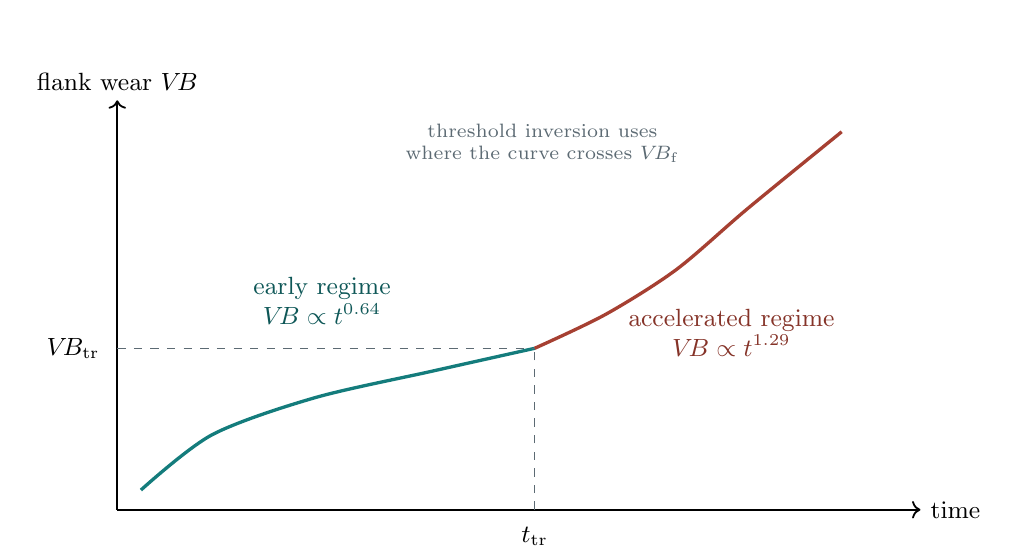
\begin{tikzpicture}[x=1cm,y=1cm]
    \draw[->,line width=0.65pt] (0,0) -- (10.2,0) node[right] {\small time};
    \draw[->,line width=0.65pt] (0,0) -- (0,5.2) node[above] {\small flank wear \(\vb\)};
    \draw[line width=1.2pt,teal] plot[smooth] coordinates {(0.3,0.25) (1.2,0.95) (2.5,1.42) (4.0,1.76) (5.3,2.05)};
    \draw[line width=1.2pt,brick] plot[smooth] coordinates {(5.3,2.05) (6.2,2.48) (7.1,3.05) (8.0,3.82) (9.2,4.8)};
    \draw[dashed,draw=muted] (5.3,0) -- (5.3,2.05);
    \draw[dashed,draw=muted] (0,2.05) -- (5.3,2.05);
    \node[font=\small,align=center,color=teal!70!black] at (2.6,2.65) {early regime\\\(\vb \propto t^{0.64}\)};
    \node[font=\small,align=center,color=brick!80!black] at (7.8,2.25) {accelerated regime\\\(\vb \propto t^{1.29}\)};
    \node[font=\small,below] at (5.3,-0.1) {\(\ttr\)};
    \node[font=\small,left] at (-0.1,2.05) {\(\vbtr\)};
    \node[font=\scriptsize,color=muted,align=center] at (5.4,4.65) {threshold inversion uses\\where the curve crosses \(\vbf\)};
  \end{tikzpicture}
  \caption{Schematic of the piecewise wear law. The transition wear is \(\vbtr=0.25~\mathrm{mm}\); early and late exponents are learned from different evidence sources.}
  \label{fig:piecewise-schematic}
\end{figure}

\subsubsection{Model Definition}

Let \(t\) denote cutting time in minutes for the simulator-scale equation, and let \(\vbf\) denote the target failure threshold. The Phase 2 model defines an early amplitude law around a reference operating point:

\begin{equation}
\phii(n,f_z,a_p) =
\left(\frac{n}{1800}\right)^{0.359967}
\left(\frac{f_z}{0.05}\right)^{3.956013}
\left(\frac{a_p}{3.0}\right)^{0.688073}.
\label{eq:condition-intensity}
\end{equation}

The early wear curve is

\begin{equation}
\vb(t) = k_{\mathrm{early}}\ \phii\ t^{\earlyexp},
\quad
k_{\mathrm{early}}=0.018580943,\quad \earlyexp=0.64.
\label{eq:early-wear}
\end{equation}

The late curve is activated after the transition wear \(\vbtr=0.25~\mathrm{mm}\). It uses an accelerated exponent \(\lateexp=1.29\) and material-aware late-stage factors. In simulator form, the model can be summarized as

\begin{equation}
\vb(t)=
\begin{cases}
k_{\mathrm{early}}\ \phii\ t^{0.64}, & \vb(t)<\vbtr,\\
\vbtr + k_{\mathrm{late}}(m)\ \phii\ (t-\ttr)^{1.29}, & \vb(t)\geq\vbtr,
\end{cases}
\label{eq:piecewise-model}
\end{equation}

where \(k_{\mathrm{late}}(m)\) is adjusted by material family. The repository records the late-stage factors as generic \(0.25\), cast iron \(0.1488\), and steel \(0.3994\). These factors should be interpreted as local calibrated simulator coefficients, not universal constants.

\subsubsection{Evidence for Exponents}

\begin{table}[!htbp]
  \centering
  \caption{Evidence used to select the Phase 2 exponents.}
  \label{tab:exponent-evidence}
  \small
  \begin{tabularx}{\textwidth}{p{2.3cm}p{2.1cm}p{2.2cm}p{2.0cm}Y}
    \toprule
    Dataset & Regime & Raw exponent & RMSE & Role in final model \\
    \midrule
    NUAA & Early & 0.6347 & 0.0211 mm & Main source for the sub-linear early wear law. \\
    PHM2010 & Early & 0.6471 & 0.0136 mm & Independent confirmation that the early exponent transfers. \\
    NASA & Late & 1.2873 & 0.0438 mm & Main source for accelerated late-stage behavior. \\
    \bottomrule
  \end{tabularx}
\end{table}

\begin{figure}[!htbp]
  \centering
  \begin{subfigure}{0.32\textwidth}
    \centering
    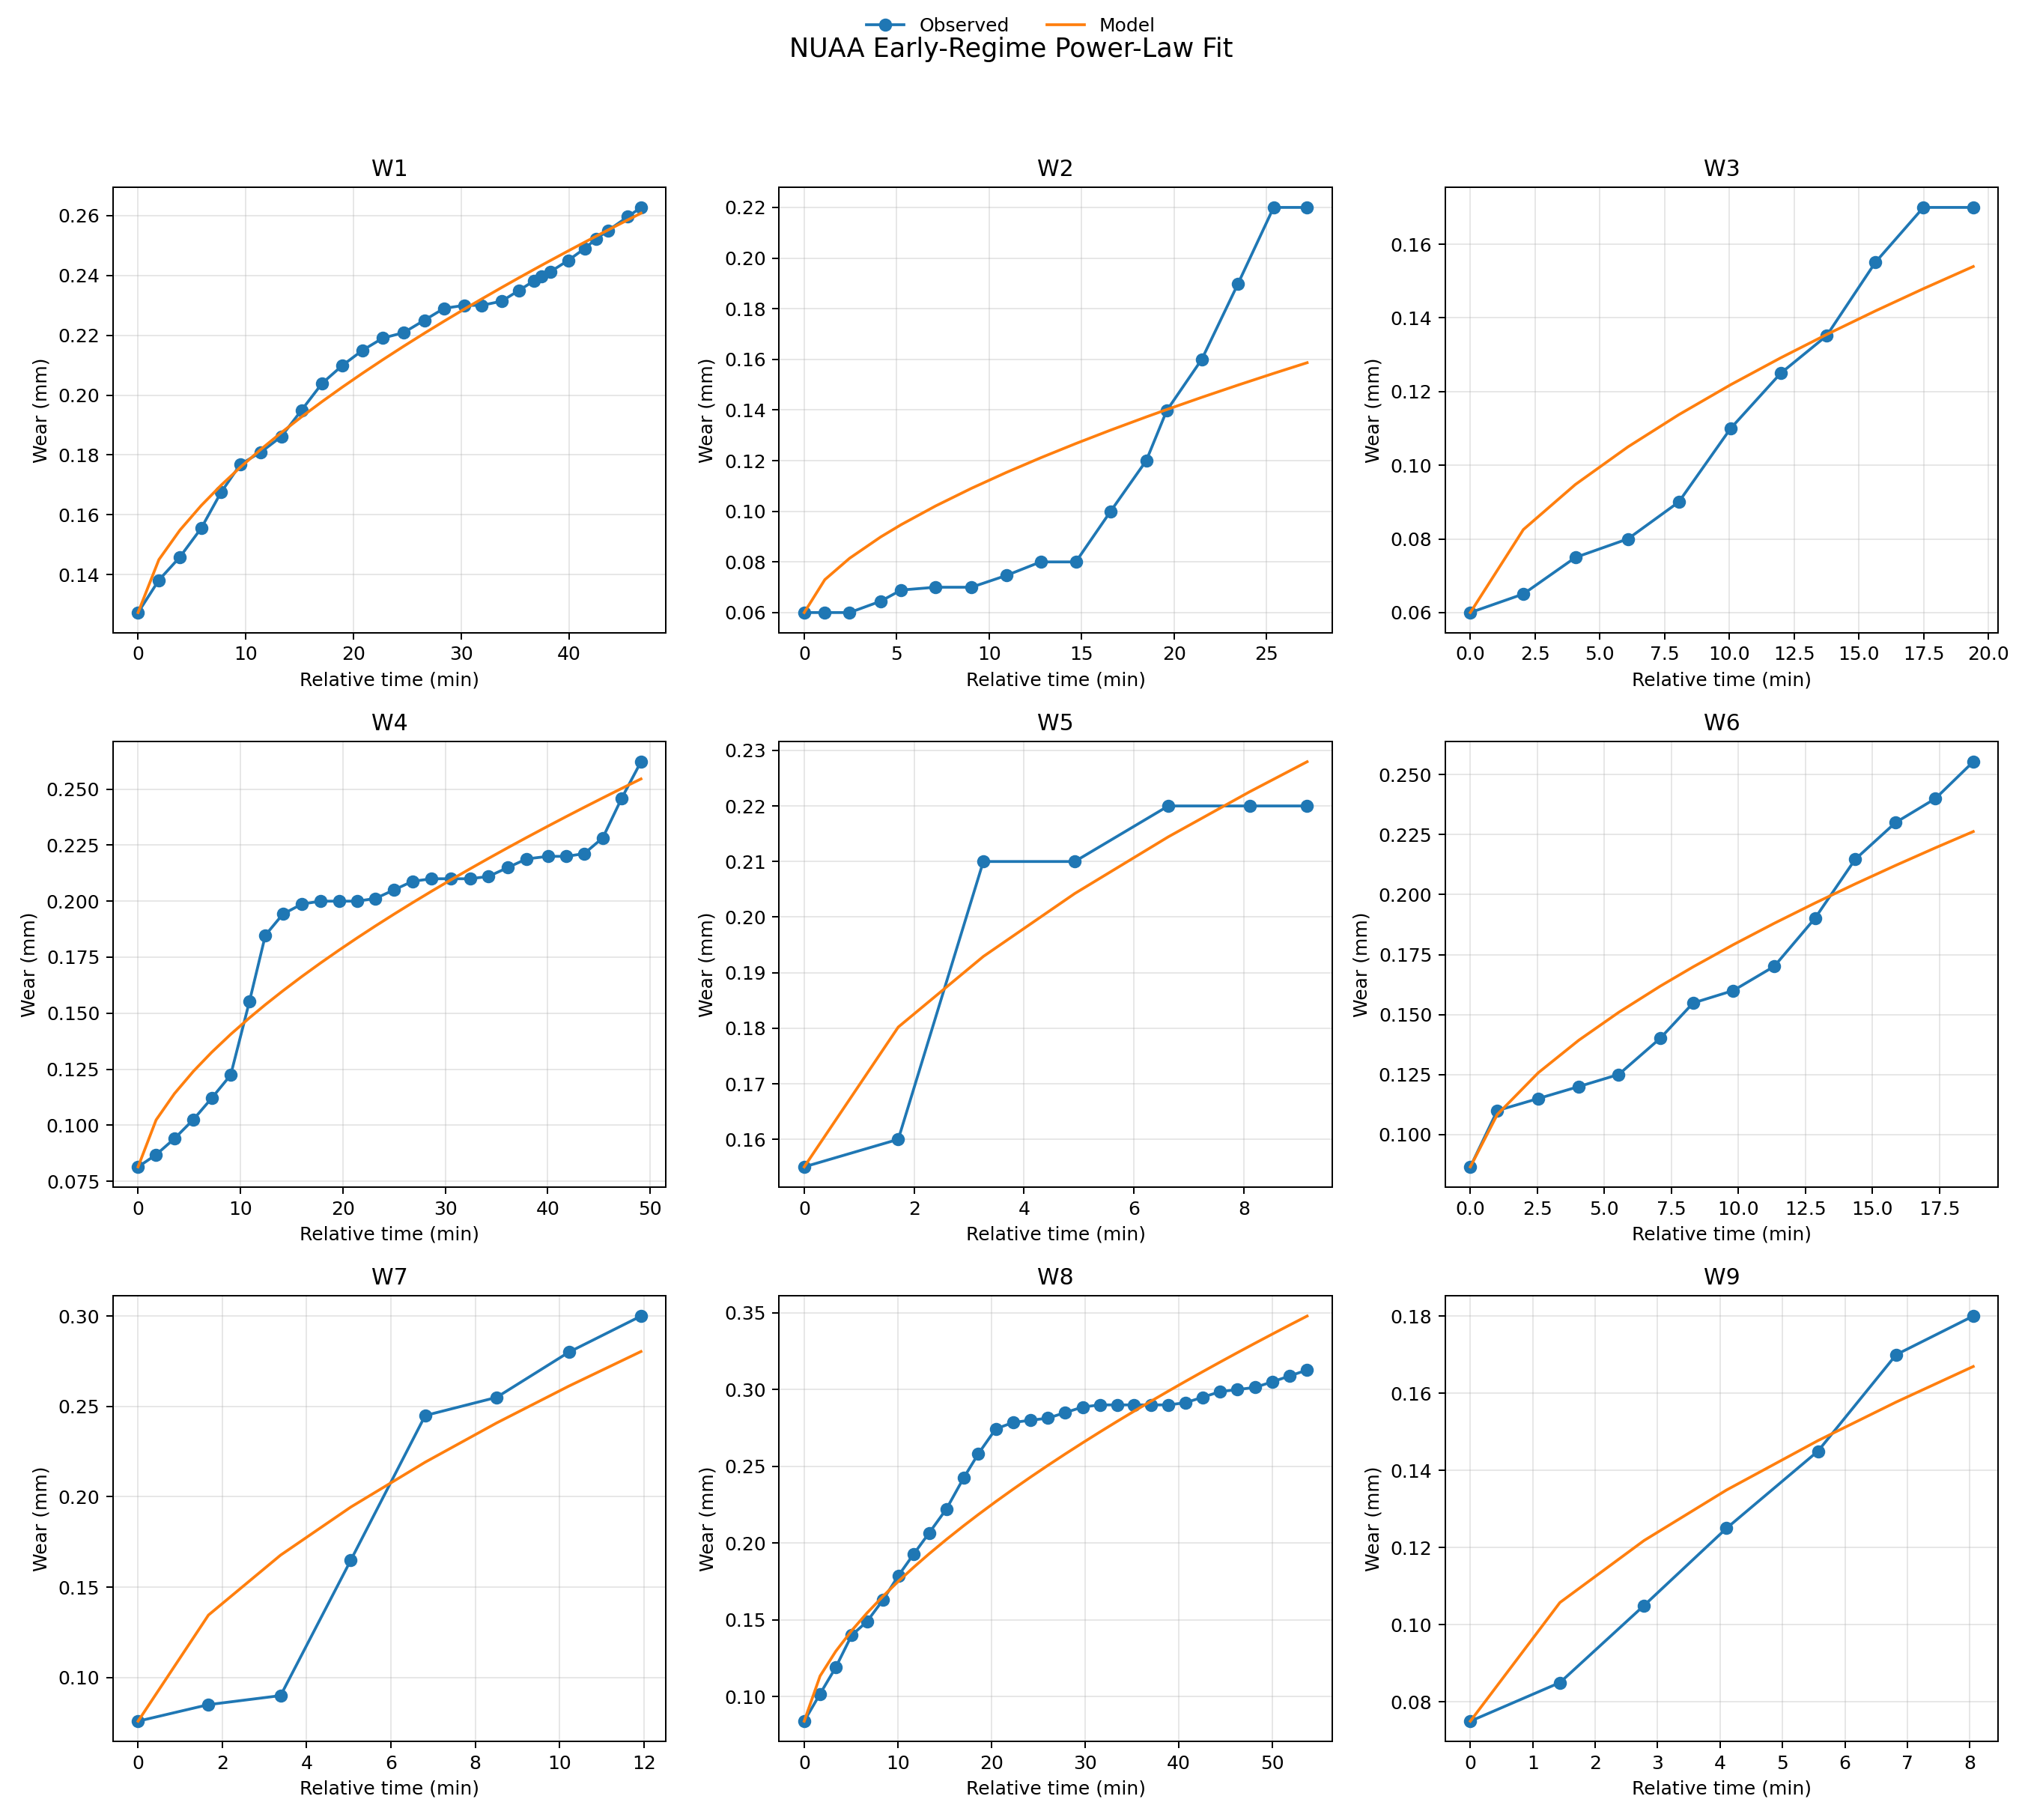
\includegraphics[width=\textwidth]{nuaa_early_regime_fit.png}
    \caption{NUAA early fit}
  \end{subfigure}
  \hfill
  \begin{subfigure}{0.32\textwidth}
    \centering
    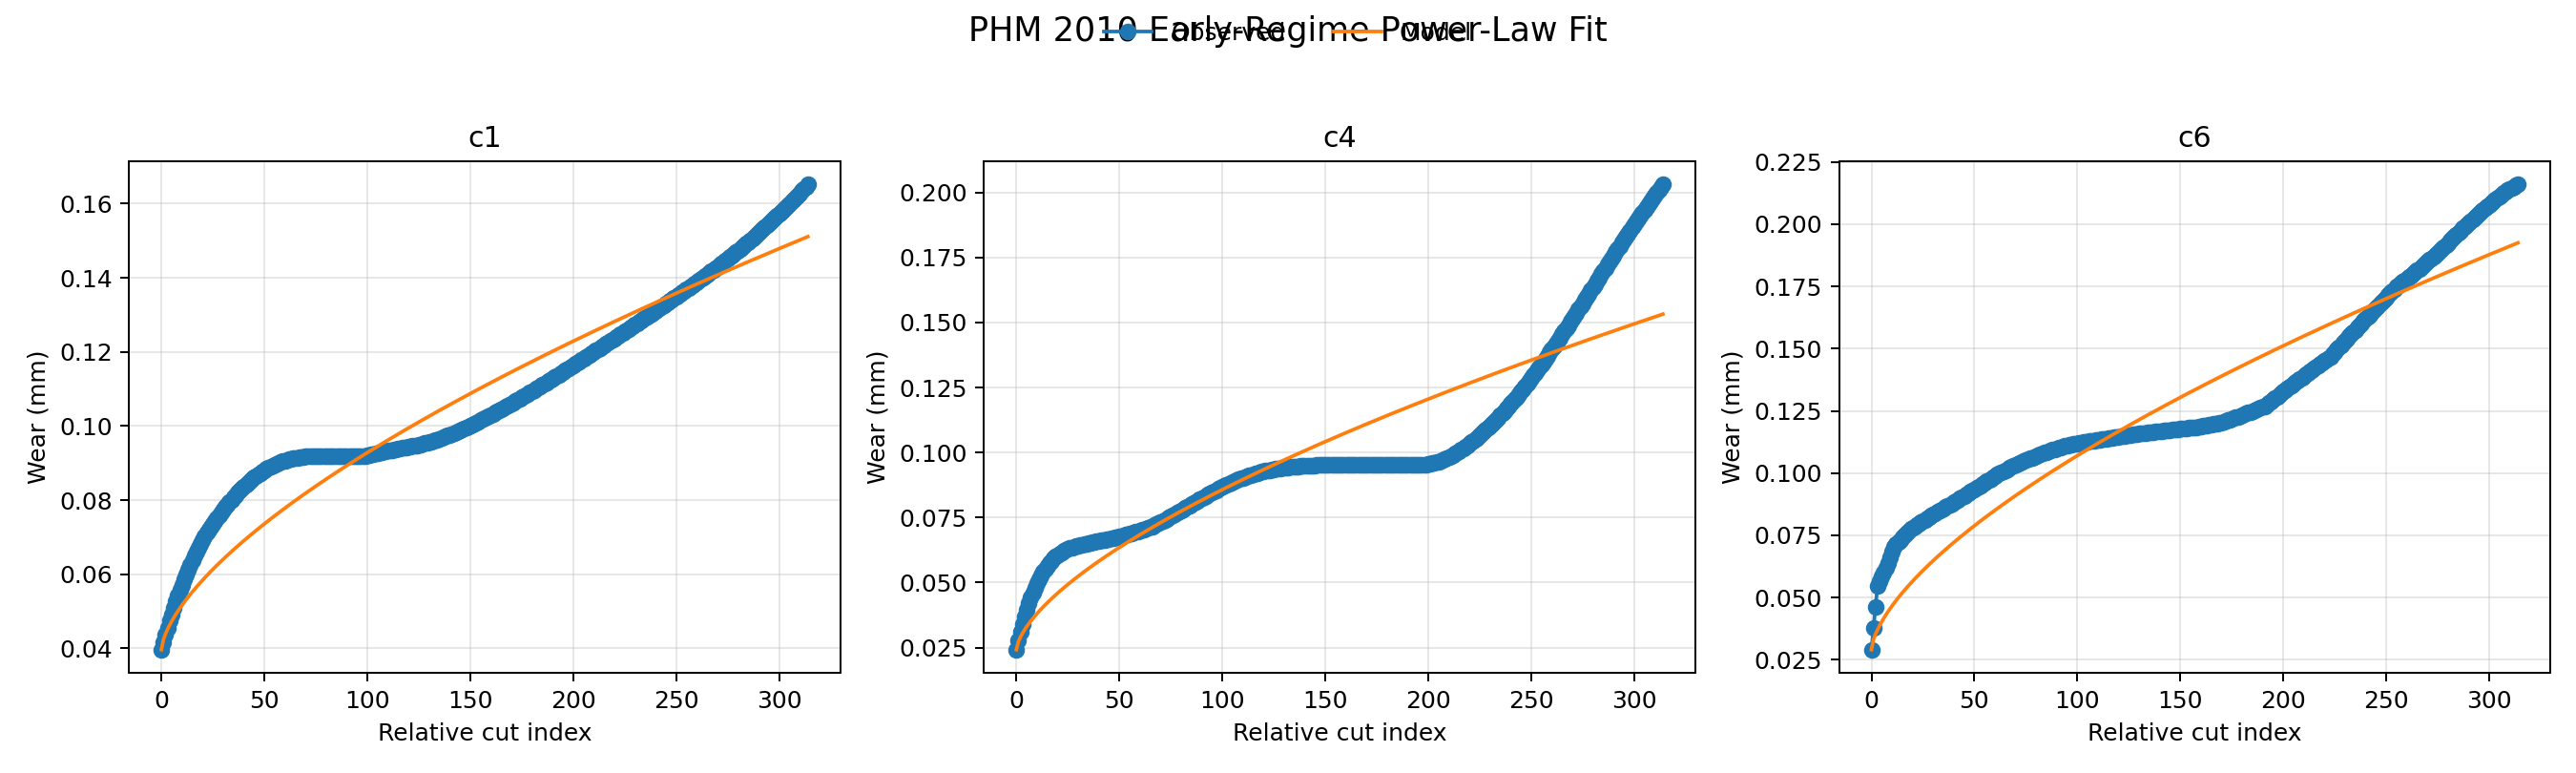
\includegraphics[width=\textwidth]{phm_early_regime_fit.png}
    \caption{PHM2010 check}
  \end{subfigure}
  \hfill
  \begin{subfigure}{0.32\textwidth}
    \centering
    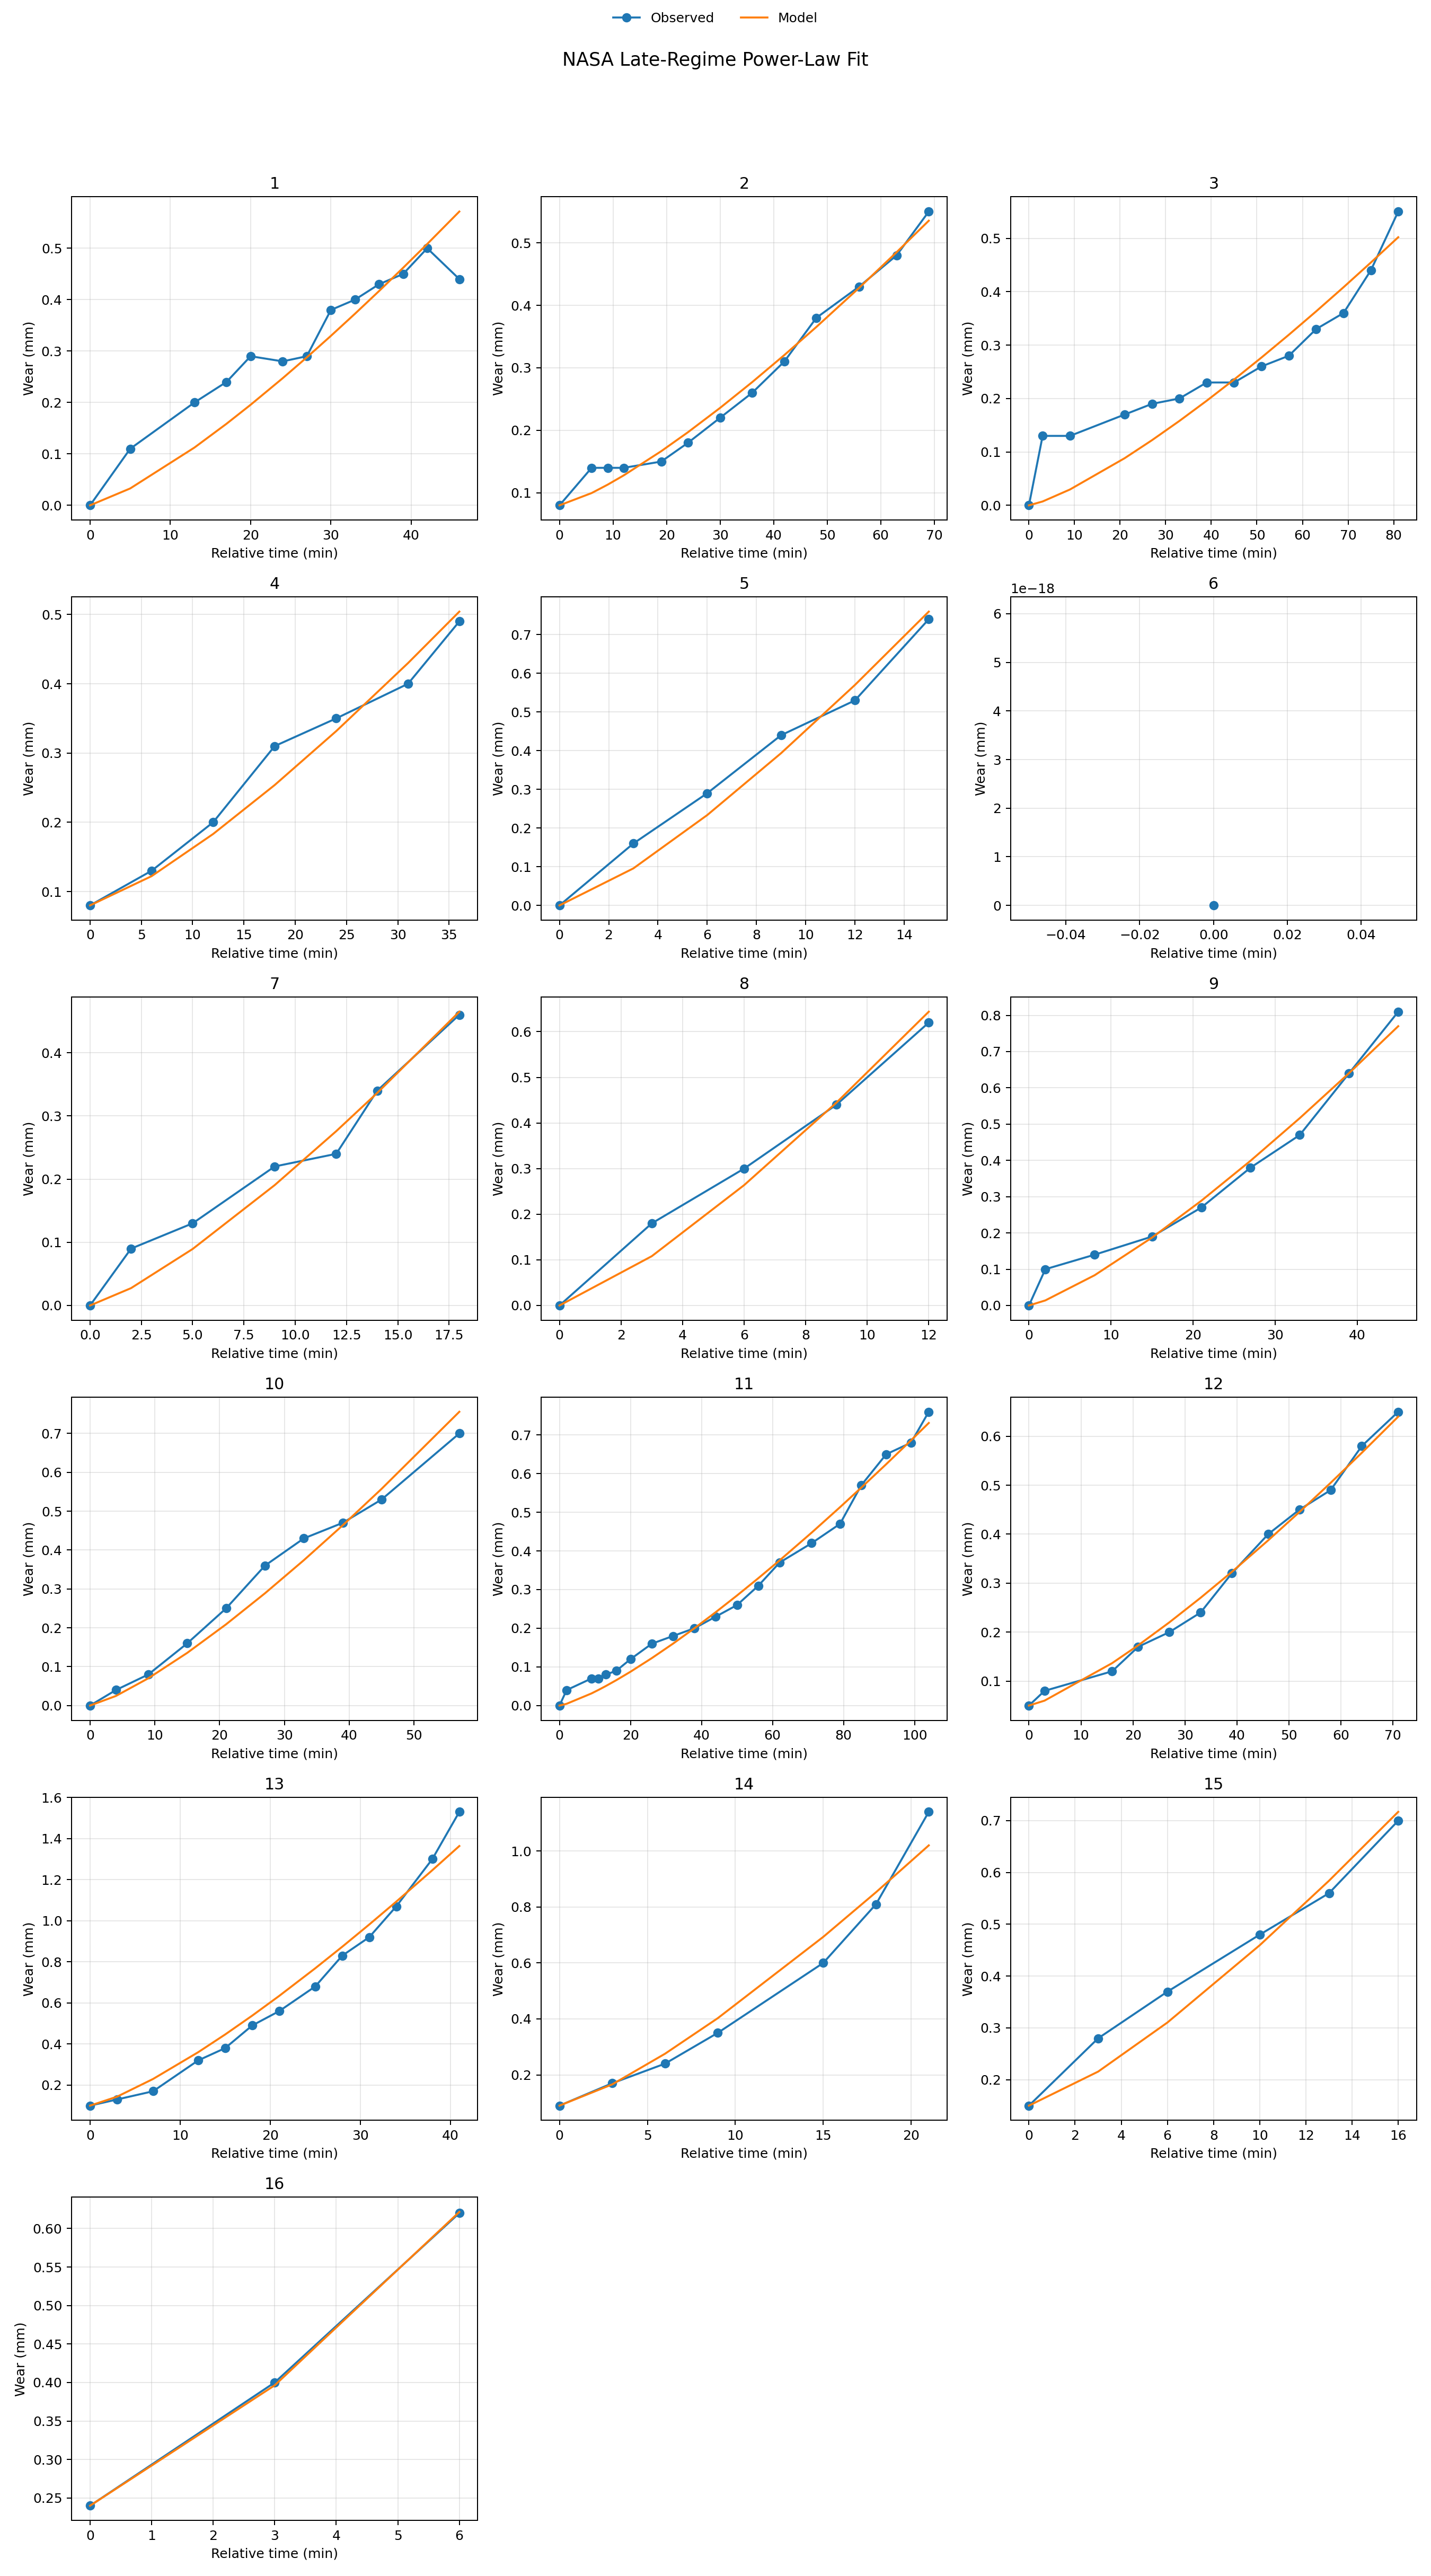
\includegraphics[width=\textwidth]{nasa_late_regime_fit.png}
    \caption{NASA late fit}
  \end{subfigure}
  \caption{The final exponents are grounded in role-specific fits rather than a single pooled curve.}
  \label{fig:regime-fits}
\end{figure}

\subsubsection{Condition Law}

The fitted process-condition intensity in \eqnref{eq:condition-intensity} is strongest in feed. That result is plausible: feed directly changes chip thickness and cutting load per tooth. Speed and depth also matter, but in the local NUAA design the feed exponent is much more stable and much larger than the others.

\begin{figure}[!htbp]
  \centering
  \begin{subfigure}{0.48\textwidth}
    \centering
    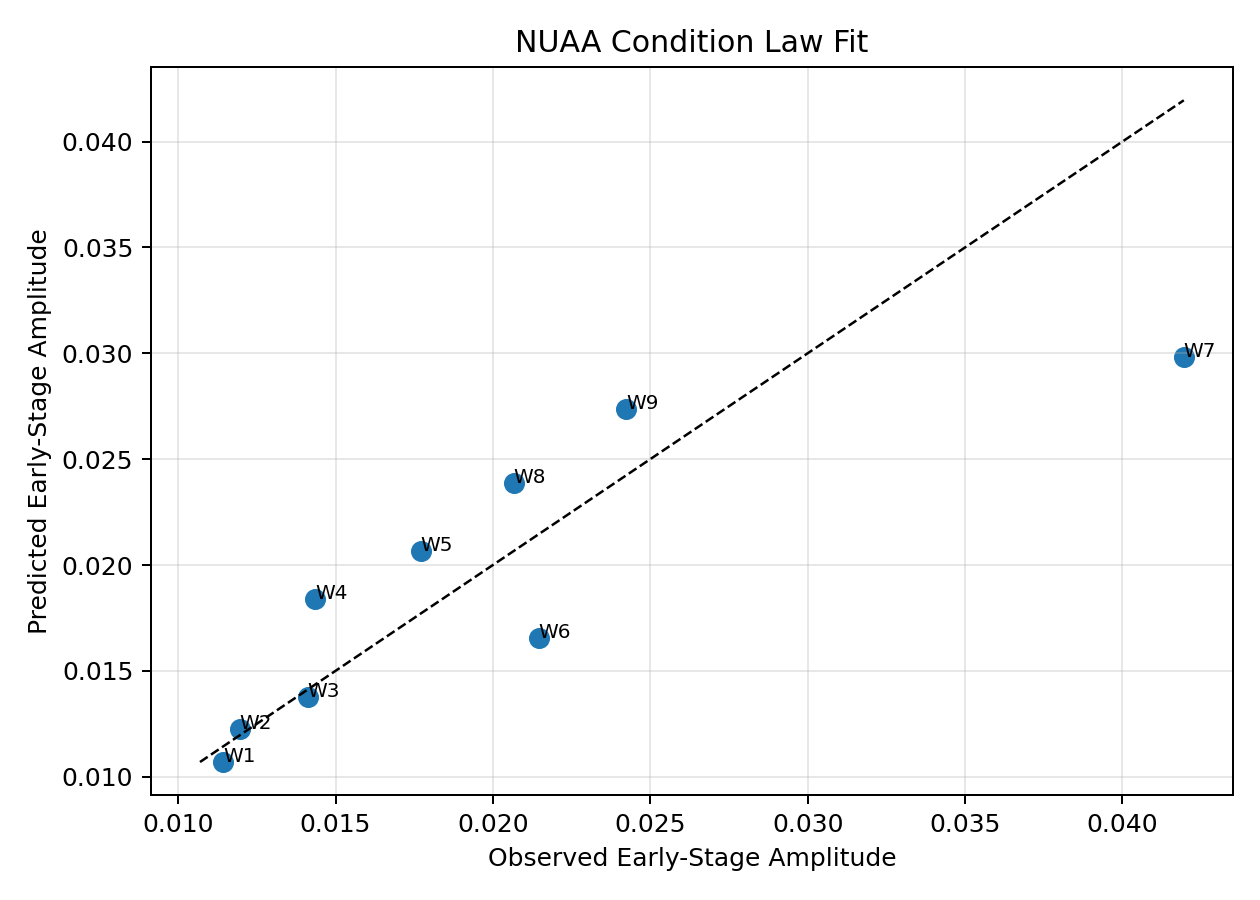
\includegraphics[width=\textwidth]{nuaa_condition_law_fit.png}
    \caption{Condition-law fit}
  \end{subfigure}
  \hfill
  \begin{subfigure}{0.48\textwidth}
    \centering
    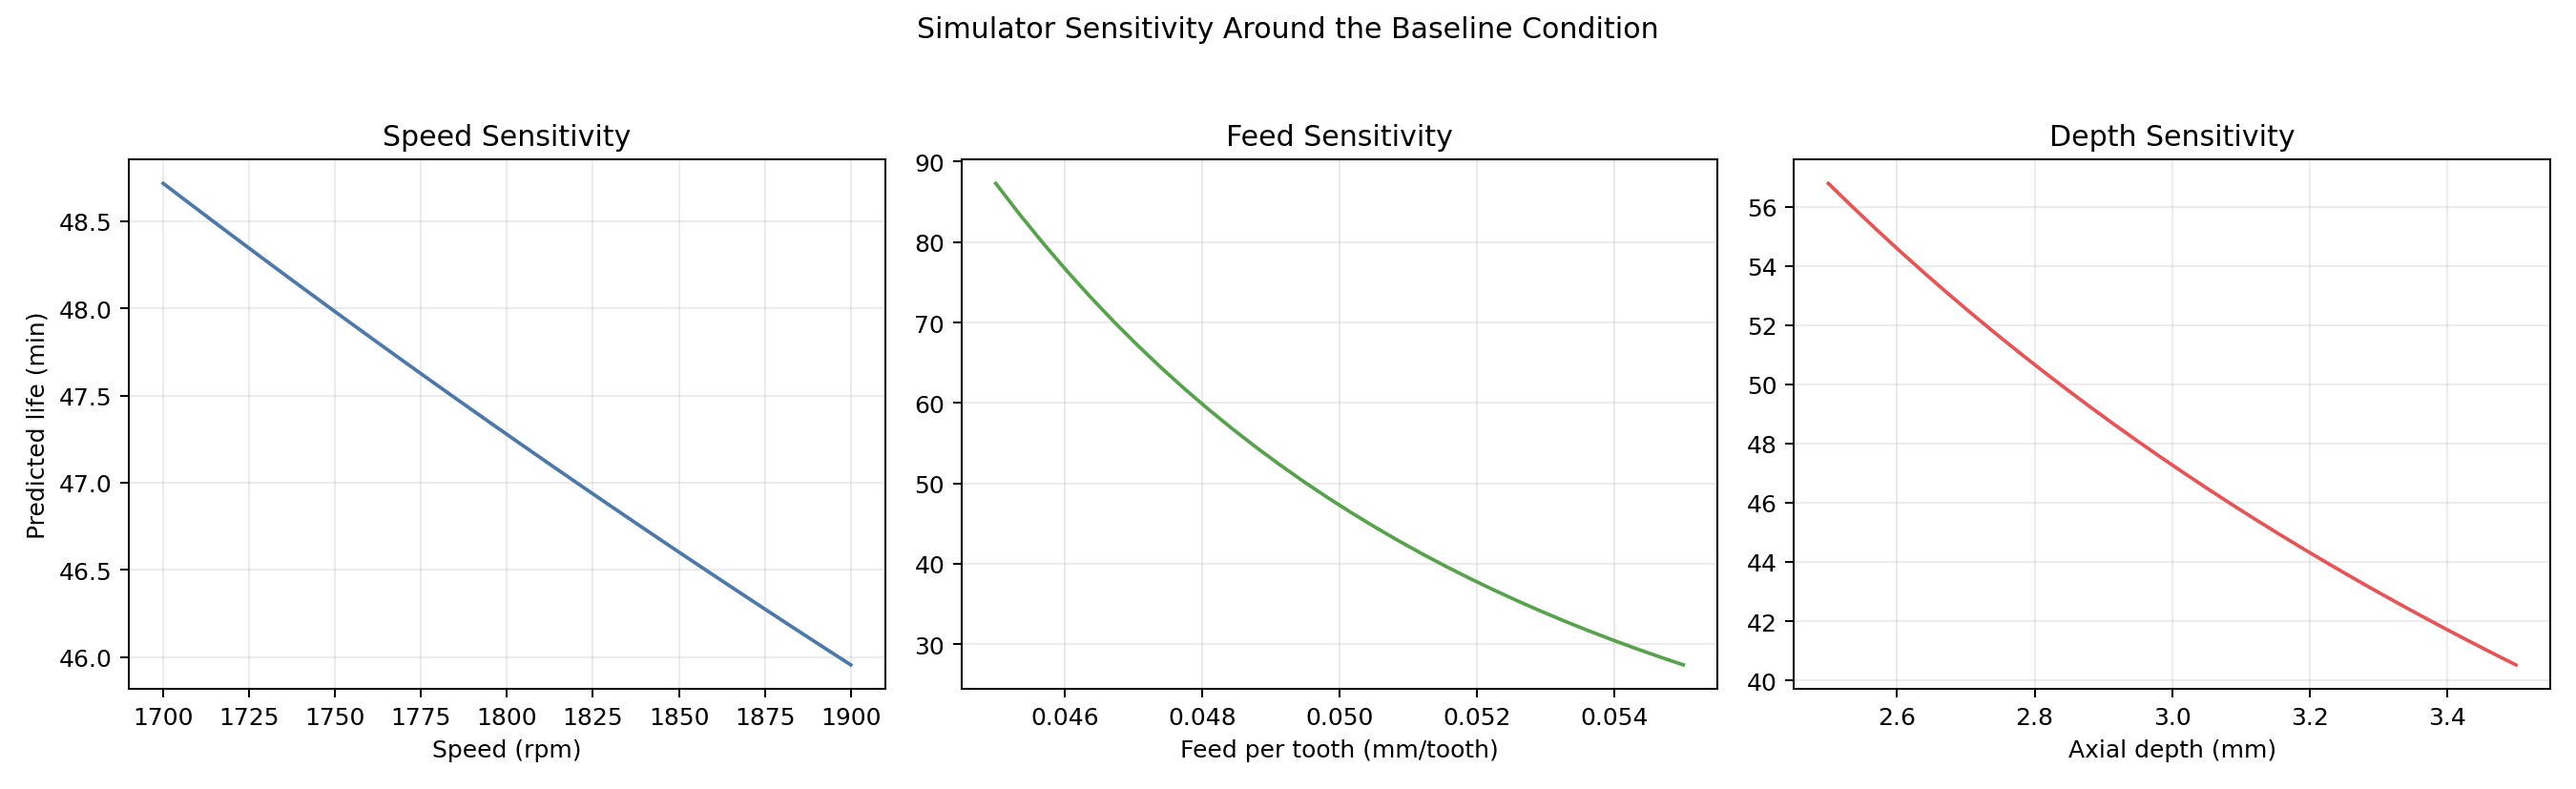
\includegraphics[width=\textwidth]{life_sensitivity_curves.png}
    \caption{Life sensitivity curves}
  \end{subfigure}
  \caption{Feed dominates the local life sensitivity, while speed and depth remain less stable because of narrower design variation and collinearity.}
  \label{fig:condition-law}
\end{figure}

\subsubsection{Material Effects}

NASA supports late-stage material comparisons, especially between cast iron and steel. The Phase 2 simulator uses this evidence to avoid treating all late-stage wear as one material-independent acceleration process.

\begin{figure}[!htbp]
  \centering
  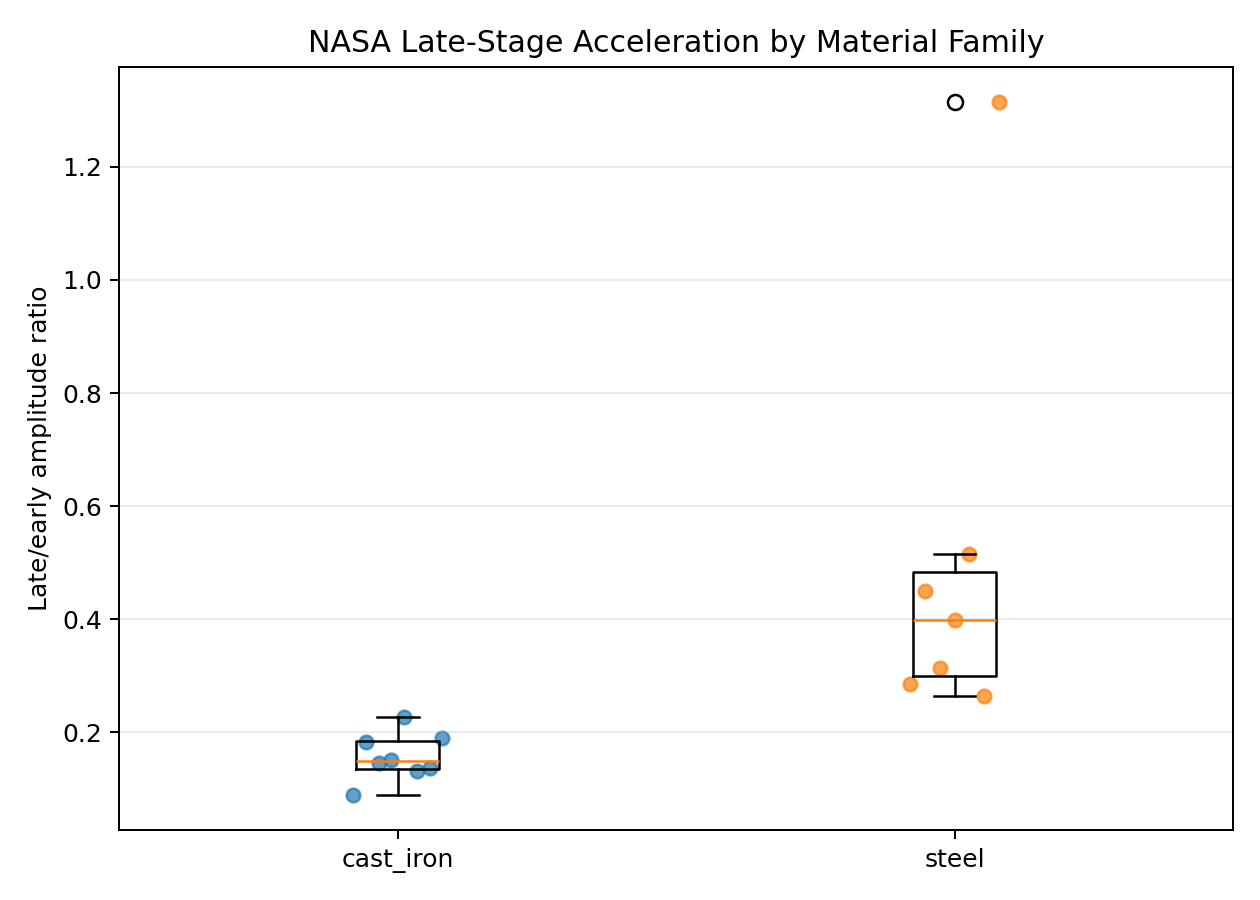
\includegraphics[width=0.78\textwidth]{nasa_late_stage_materials.png}
  \caption{NASA late-stage material behavior. Steel shows a stronger late-stage wear factor than cast iron in the local model.}
  \label{fig:nasa-materials}
\end{figure}

\section{Results and Discussions}

\subsection{Cross-Dataset Baselines}

\subsubsection{Regression and Failure Classification}

The cross-dataset pipeline evaluates Ridge, Random Forest, and Gradient Boosting style models with grouped validation. Grouped validation is important because adjacent samples from the same cutter or case are not independent deployment tests. The goal is to estimate whether a model transfers to unseen experiments, not whether it can interpolate adjacent points within the same trajectory.

\begin{table}[!htbp]
  \centering
  \caption{Cross-dataset wear regression and failure classification results.}
  \label{tab:cross-dataset-metrics}
  \small
  \begin{tabular}{lrrrrrr}
    \toprule
    Dataset & Samples & Groups & Features & Best regressor & RMSE & ROC-AUC \\
    \midrule
    PHM2010 & 945 & 3 & 105 & Random Forest & 0.0181 & 0.9671 \\
    NASA & 146 & 16 & 94 & Ridge & 0.1728 & 0.9141 \\
    UniWear & 649 & 12 & 46 & Ridge & 0.0475 & 0.7350 \\
    \bottomrule
  \end{tabular}
\end{table}

\begin{figure}[!htbp]
  \centering
  \begin{subfigure}{0.48\textwidth}
    \centering
    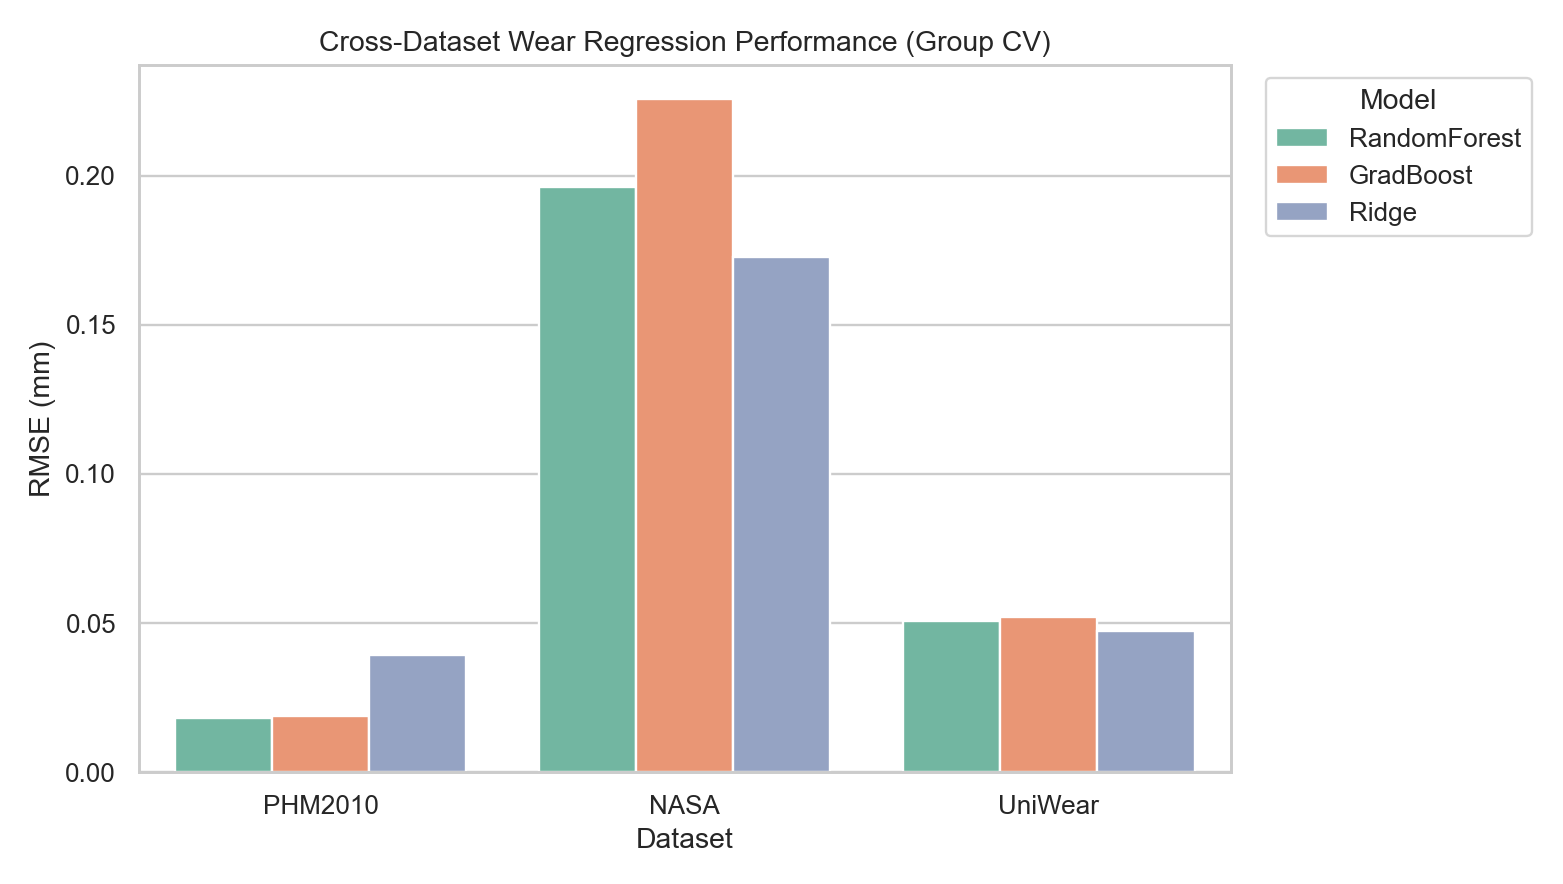
\includegraphics[width=\textwidth]{cross_dataset_rmse_comparison.png}
    \caption{Regression RMSE}
  \end{subfigure}
  \hfill
  \begin{subfigure}{0.48\textwidth}
    \centering
    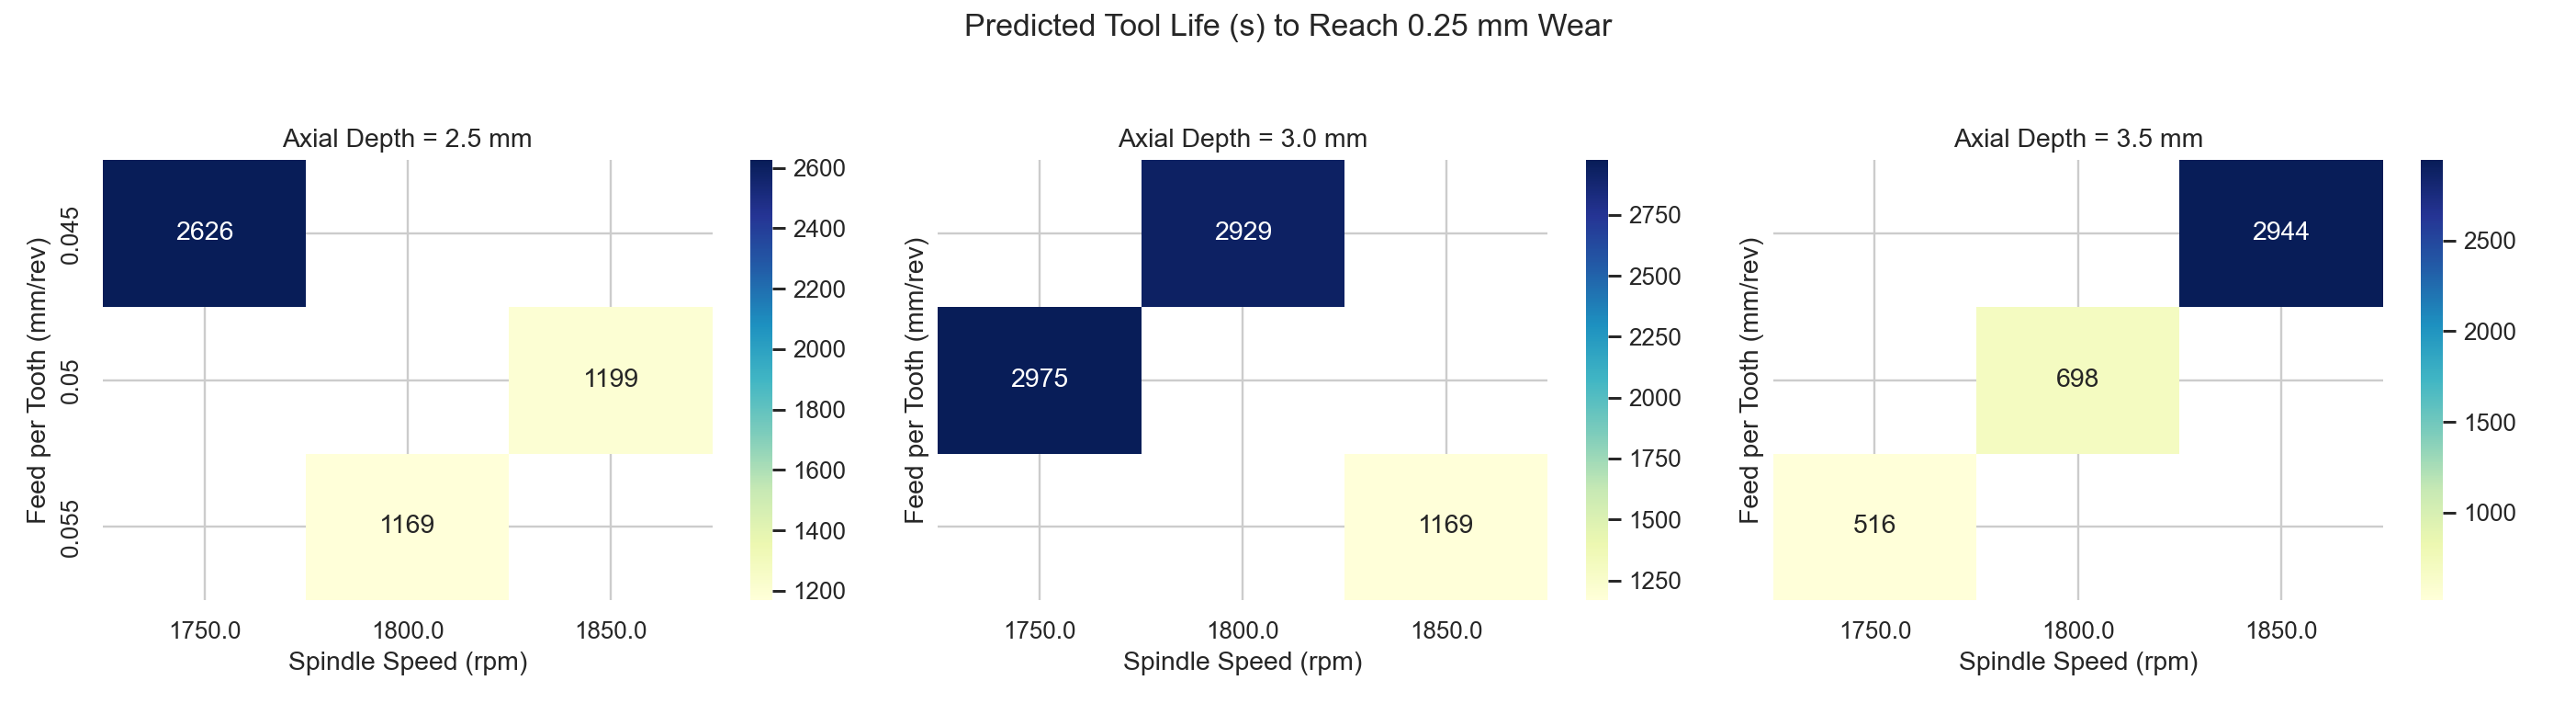
\includegraphics[width=\textwidth]{nuaa_life_heatmap.png}
    \caption{NUAA life heatmap}
  \end{subfigure}
  \caption{Cross-dataset baselines and NUAA process-condition sensitivity.}
  \label{fig:cross-dataset-baselines}
\end{figure}

\subsubsection{Per-Dataset Health Markers}

The failure-marker plots show a practical theme: failure labels are usually preceded by increasing signal energy, dispersion, or impulsiveness, but the exact feature family varies by dataset. This is consistent with machining physics. Tool wear changes the chip formation process, contact geometry, friction, heat generation, and dynamic stiffness; the resulting evidence can appear in vibration, acoustic emission, force/current, or derived frequency features depending on available sensors.

\begin{figure}[!htbp]
  \centering
  \begin{subfigure}{0.32\textwidth}
    \centering
    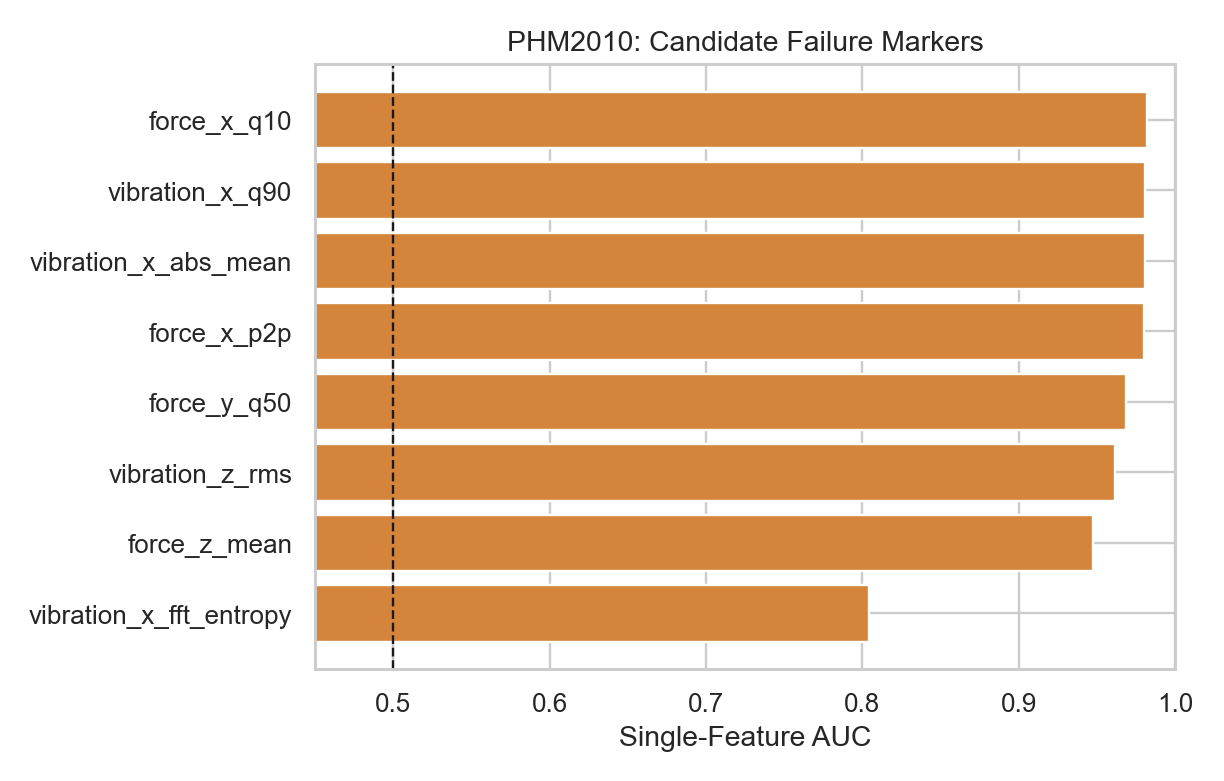
\includegraphics[width=\textwidth]{phm2010_failure_markers.png}
    \caption{PHM2010}
  \end{subfigure}
  \hfill
  \begin{subfigure}{0.32\textwidth}
    \centering
    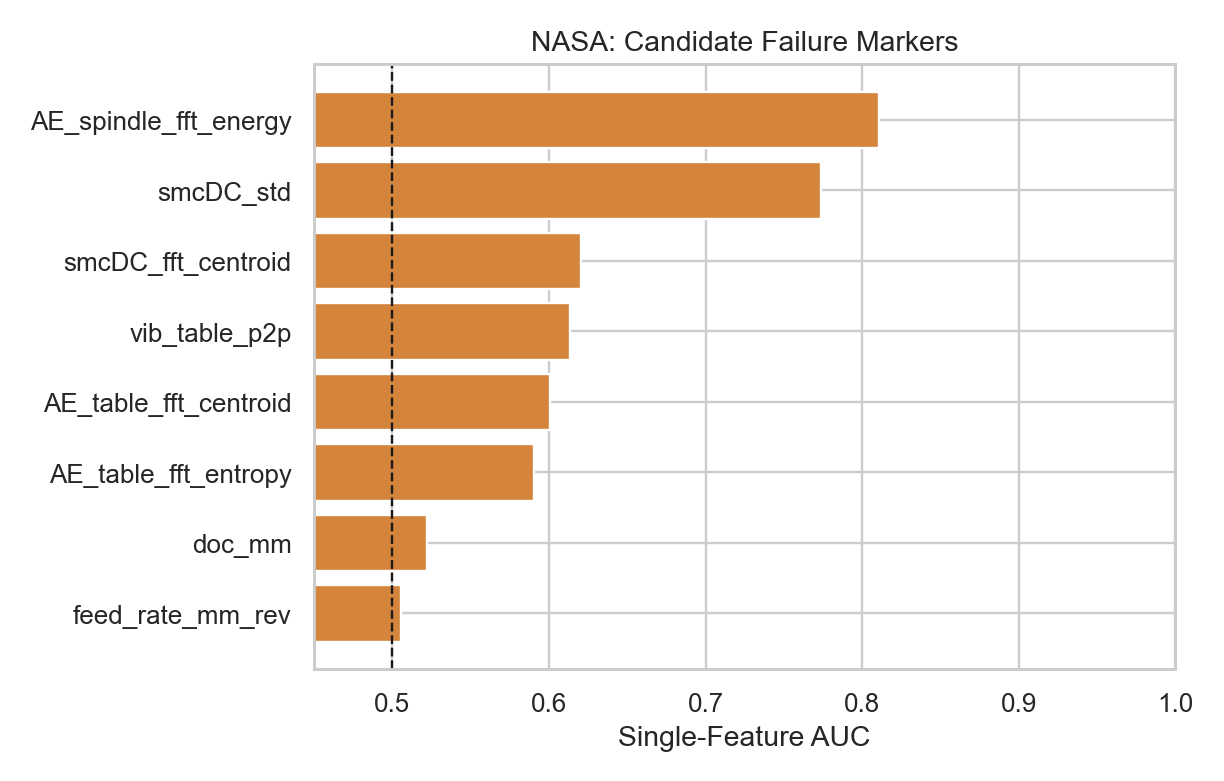
\includegraphics[width=\textwidth]{nasa_failure_markers.png}
    \caption{NASA}
  \end{subfigure}
  \hfill
  \begin{subfigure}{0.32\textwidth}
    \centering
    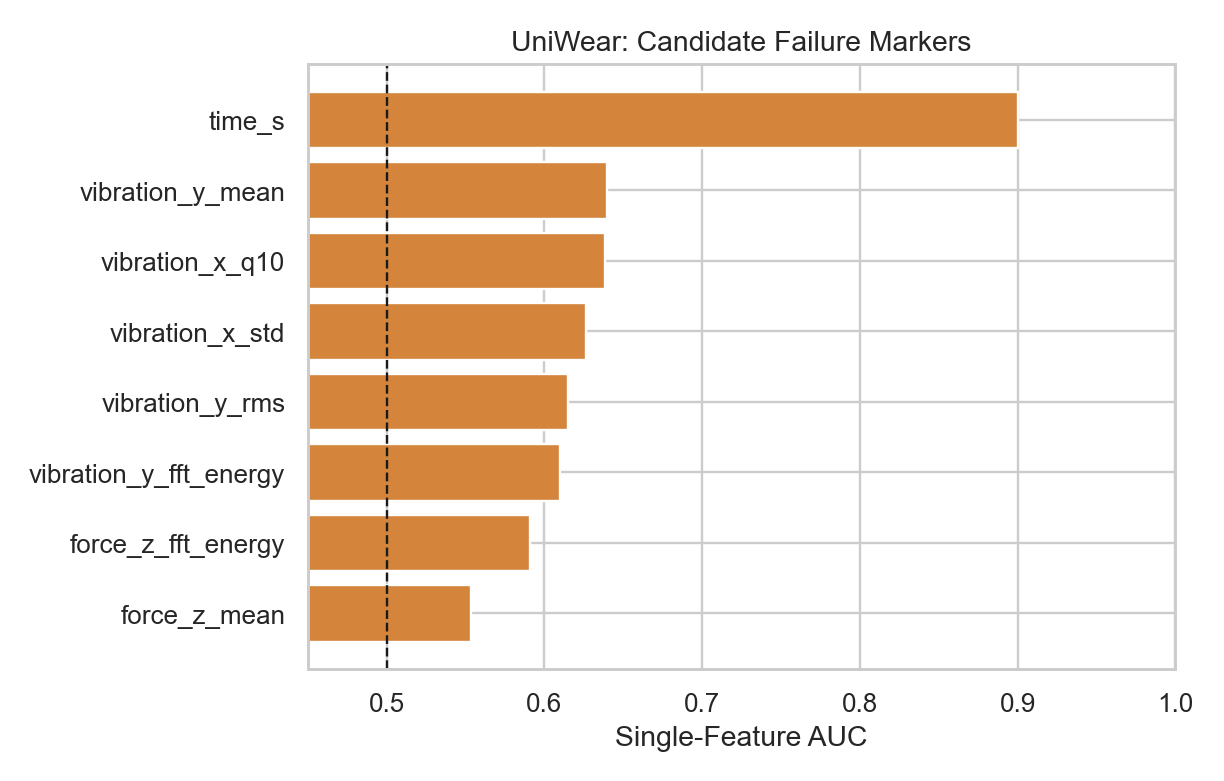
\includegraphics[width=\textwidth]{uniwear_failure_markers.png}
    \caption{UniWear}
  \end{subfigure}
  \caption{Failure-marker summaries across datasets. The plots support the use of energy, dispersion, crest, and modal frequency indicators as health signals.}
  \label{fig:failure-markers}
\end{figure}

\subsection{Uncertainty, Calibration, and Residuals}

\subsubsection{Bootstrap Coefficient Stability}

The extended research pass bootstraps the NUAA condition law with valid-design filtering. This is important because small experimental designs can produce rank-deficient or unstable resamples. The bootstrap results show a stable feed exponent, while speed and depth remain more uncertain.

\begin{table}[!htbp]
  \centering
  \caption{Bootstrap coefficient summary for the NUAA condition law.}
  \label{tab:bootstrap-coefficients}
  \small
  \begin{tabular}{lrrr}
    \toprule
    Quantity & 2.5\% & Median & 97.5\% \\
    \midrule
    \(k_{\mathrm{early}}\) & 0.01558 & 0.01783 & 0.02183 \\
    Speed exponent & -7.49808 & 1.16739 & 8.04424 \\
    Feed exponent & 2.04563 & 3.99243 & 6.68021 \\
    Depth exponent & -0.59012 & 0.51957 & 1.92473 \\
    Amplitude \(R^2\) & -- & 0.89715 & -- \\
    \bottomrule
  \end{tabular}
\end{table}

\begin{figure}[!htbp]
  \centering
  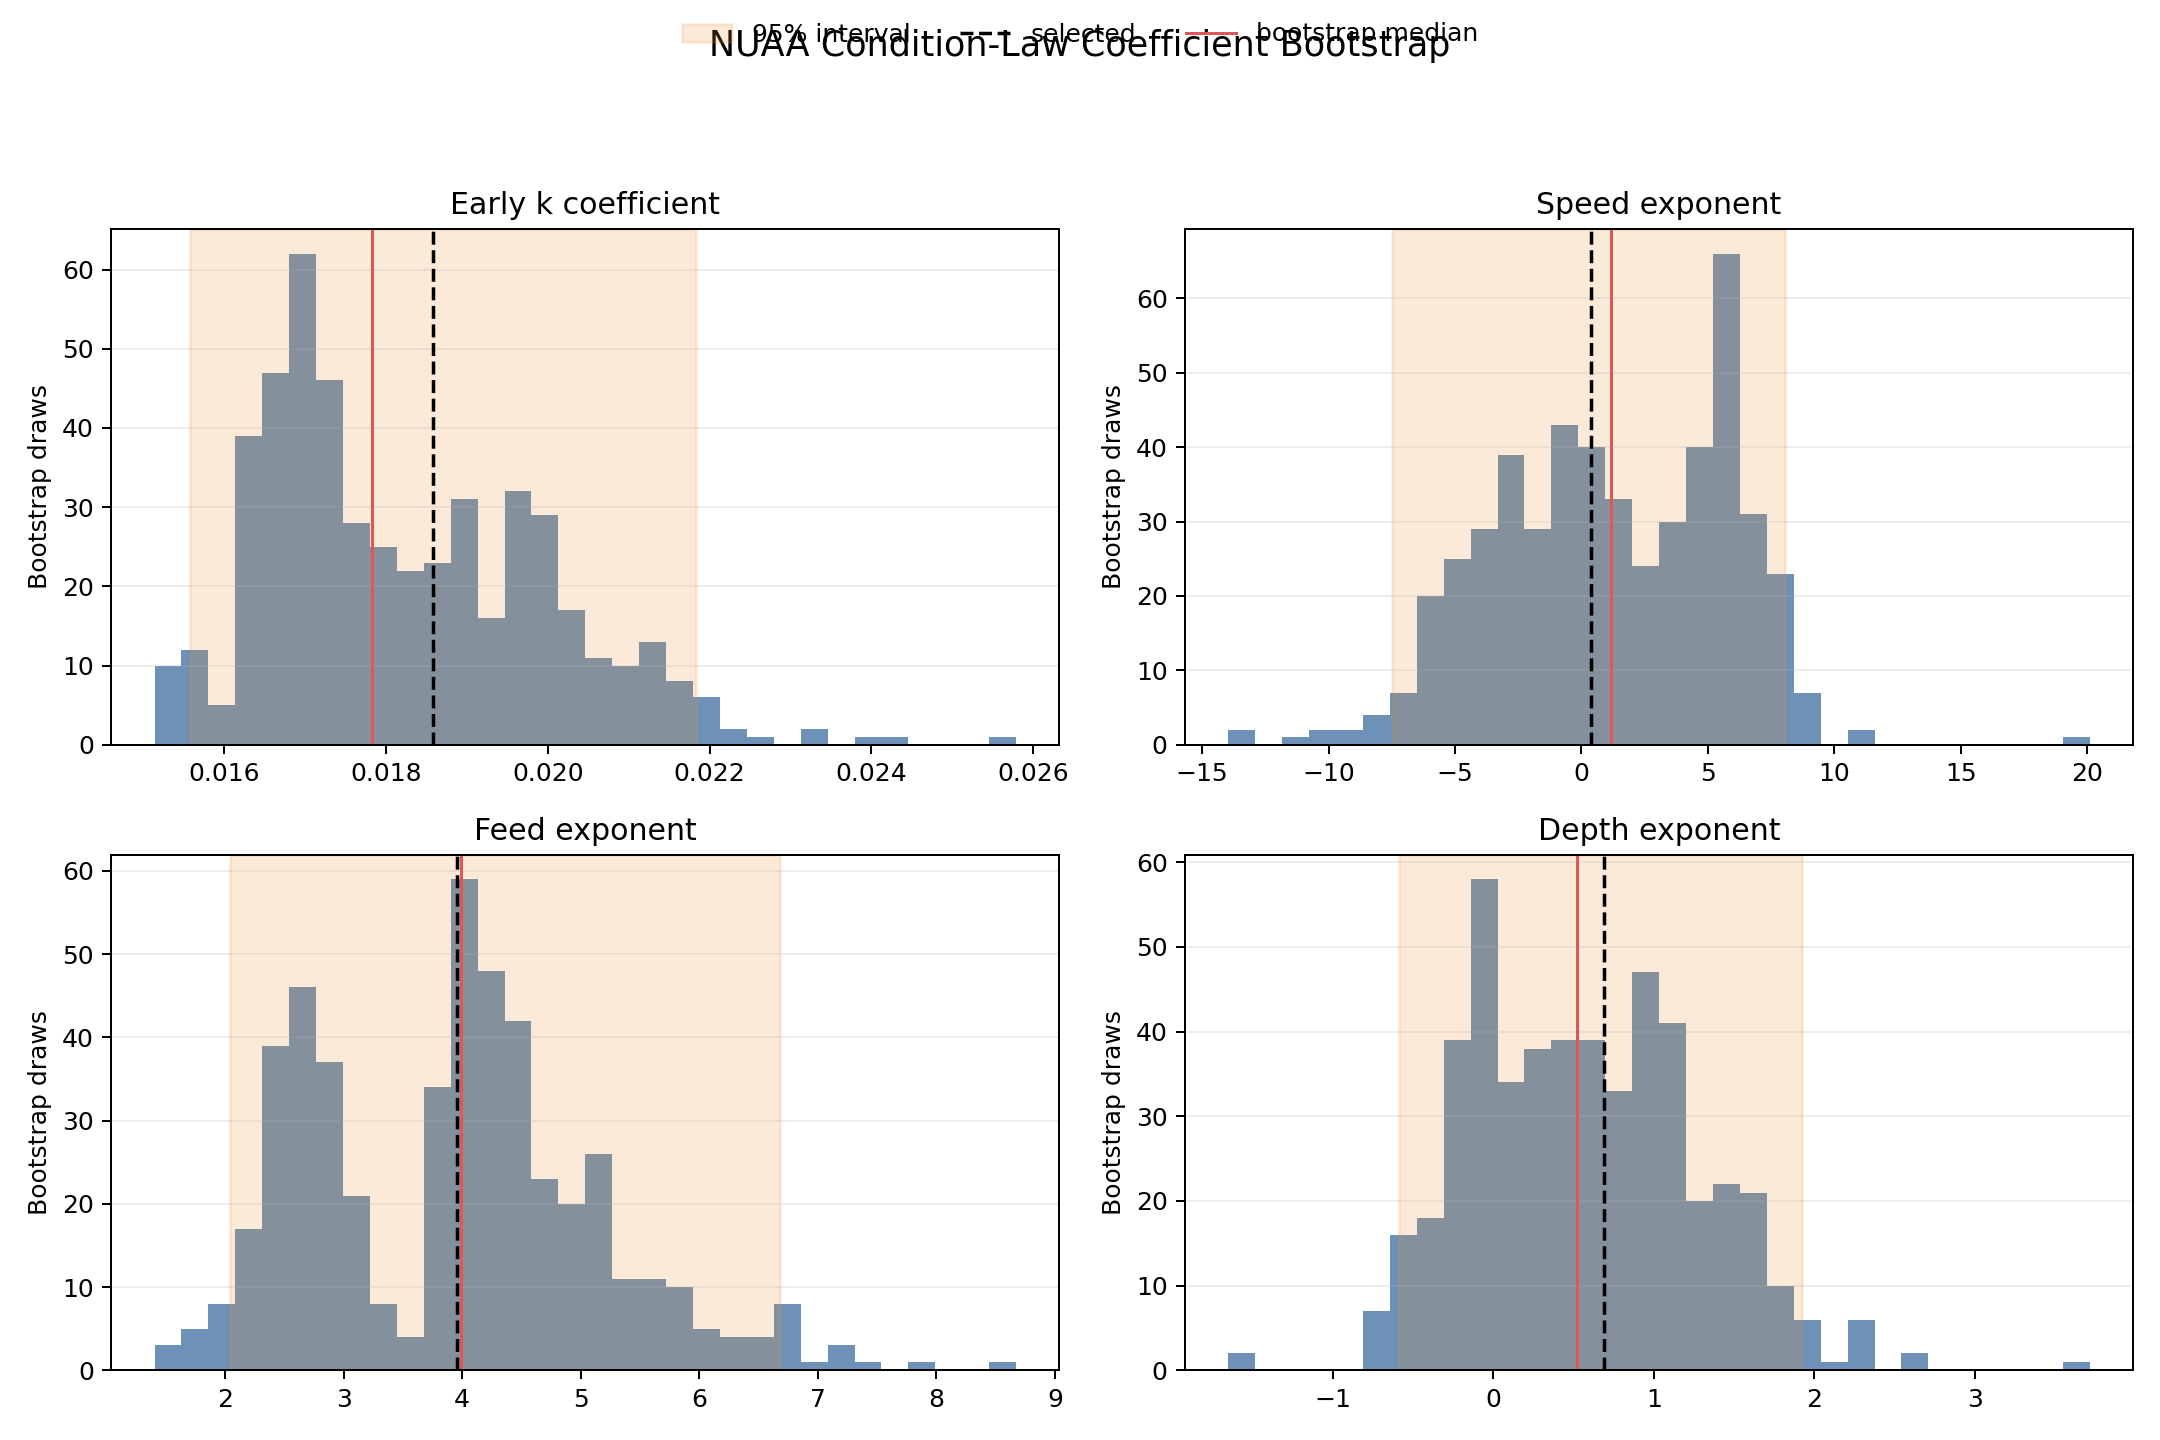
\includegraphics[width=0.82\textwidth]{condition_coefficient_bootstrap.png}
  \caption{Bootstrap distributions for condition-law coefficients. Feed is the most consistently identified operating variable in the local design.}
  \label{fig:bootstrap-coefficients}
\end{figure}

\subsubsection{Life Prediction Intervals}

The bootstrap draws were propagated into low-load, baseline, and high-load life scenarios. The result gives a practical load comparison: the baseline median life is about \textbf{50.2 minutes}, the low-load condition extends median life to about \textbf{103.6 minutes}, and the high-load condition compresses median life to about \textbf{25.0 minutes}.

\begin{table}[!htbp]
  \centering
  \caption{Bootstrap life prediction intervals.}
  \label{tab:life-intervals}
  \small
  \begin{tabular}{lrrrrrr}
    \toprule
    Scenario & Speed & Feed & Depth & 2.5\% & Median & 97.5\% \\
    \midrule
    Low load & 1750 & 0.045 & 2.5 & 59.797 & 103.644 & 247.675 \\
    Baseline & 1800 & 0.050 & 3.0 & 37.422 & 50.227 & 61.177 \\
    High load & 1850 & 0.055 & 3.5 & 11.514 & 24.987 & 38.046 \\
    \bottomrule
  \end{tabular}
\end{table}

\begin{figure}[!htbp]
  \centering
  \begin{subfigure}{0.48\textwidth}
    \centering
    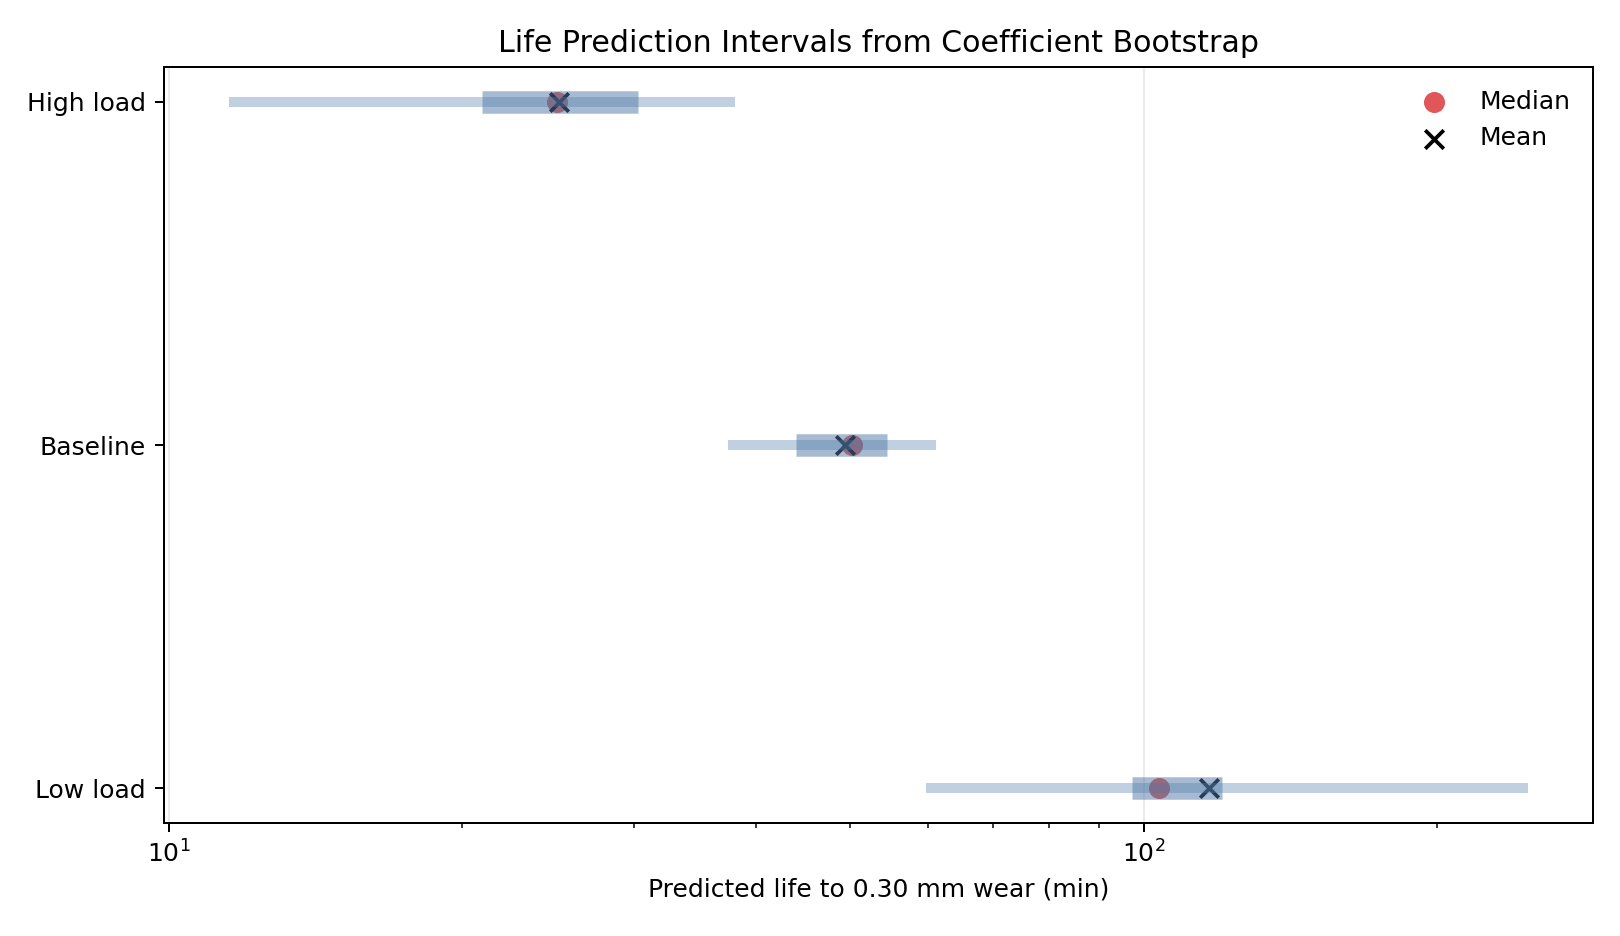
\includegraphics[width=\textwidth]{life_prediction_intervals.png}
    \caption{Interval estimates}
  \end{subfigure}
  \hfill
  \begin{subfigure}{0.48\textwidth}
    \centering
    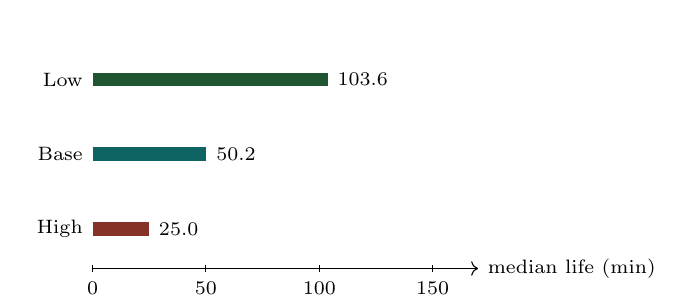
\begin{tikzpicture}[x=0.72cm,y=1cm]
      \draw[->] (0,0) -- (6.8,0) node[right] {\scriptsize median life (min)};
      \foreach \x/\lab in {0/0,2/50,4/100,6/150} {
        \draw (\x,0.05) -- (\x,-0.05) node[below,font=\scriptsize] {\lab};
      }
      \draw[line width=5pt,green!70!black] (0,2.4) -- (4.15,2.4);
      \draw[line width=5pt,teal!80!black] (0,1.45) -- (2.01,1.45);
      \draw[line width=5pt,brick!80!black] (0,0.5) -- (1.0,0.5);
      \node[left,font=\scriptsize] at (0,2.4) {Low};
      \node[left,font=\scriptsize] at (0,1.45) {Base};
      \node[left,font=\scriptsize] at (0,0.5) {High};
      \node[right,font=\scriptsize] at (4.15,2.4) {103.6};
      \node[right,font=\scriptsize] at (2.01,1.45) {50.2};
      \node[right,font=\scriptsize] at (1.0,0.5) {25.0};
    \end{tikzpicture}
    \caption{Load comparison sketch}
  \end{subfigure}
  \caption{Load changes produce large predicted life changes; the high-load condition roughly halves baseline life in the bootstrap median.}
  \label{fig:life-intervals}
\end{figure}

\subsubsection{Early Calibration Result}

The extended research pass tested whether early observations from each run could calibrate the global equation through a per-run multiplier. This is a reasonable idea: if the first few points indicate that a tool is wearing faster than expected, a calibrated forecast might improve the remaining trajectory. The local NUAA holdout result was negative. For the tested early cutoffs, calibrated forecasts had worse median holdout RMSE than the uncalibrated global model.

\begin{table}[!htbp]
  \centering
  \caption{NUAA early-window calibration holdout. Lower RMSE is better.}
  \label{tab:calibration-holdout}
  \small
  \begin{tabular}{rrrrr}
    \toprule
    Cutoff fraction & Experiments & Median points & Calibrated RMSE & Uncalibrated RMSE \\
    \midrule
    0.25 & 7 & 5.0 & 0.05045 & 0.04047 \\
    0.40 & 8 & 4.5 & 0.04750 & 0.02508 \\
    0.60 & 8 & 7.0 & 0.04230 & 0.02819 \\
    \bottomrule
  \end{tabular}
\end{table}

This result should stay in the paper because it prevents an overly optimistic simulator story. The current global model is more stable than short-window multiplicative recalibration. In future work, calibration should use a structured Bayesian update, monotonic constraints, or a state-space model instead of a free scalar multiplier.

\begin{figure}[!htbp]
  \centering
  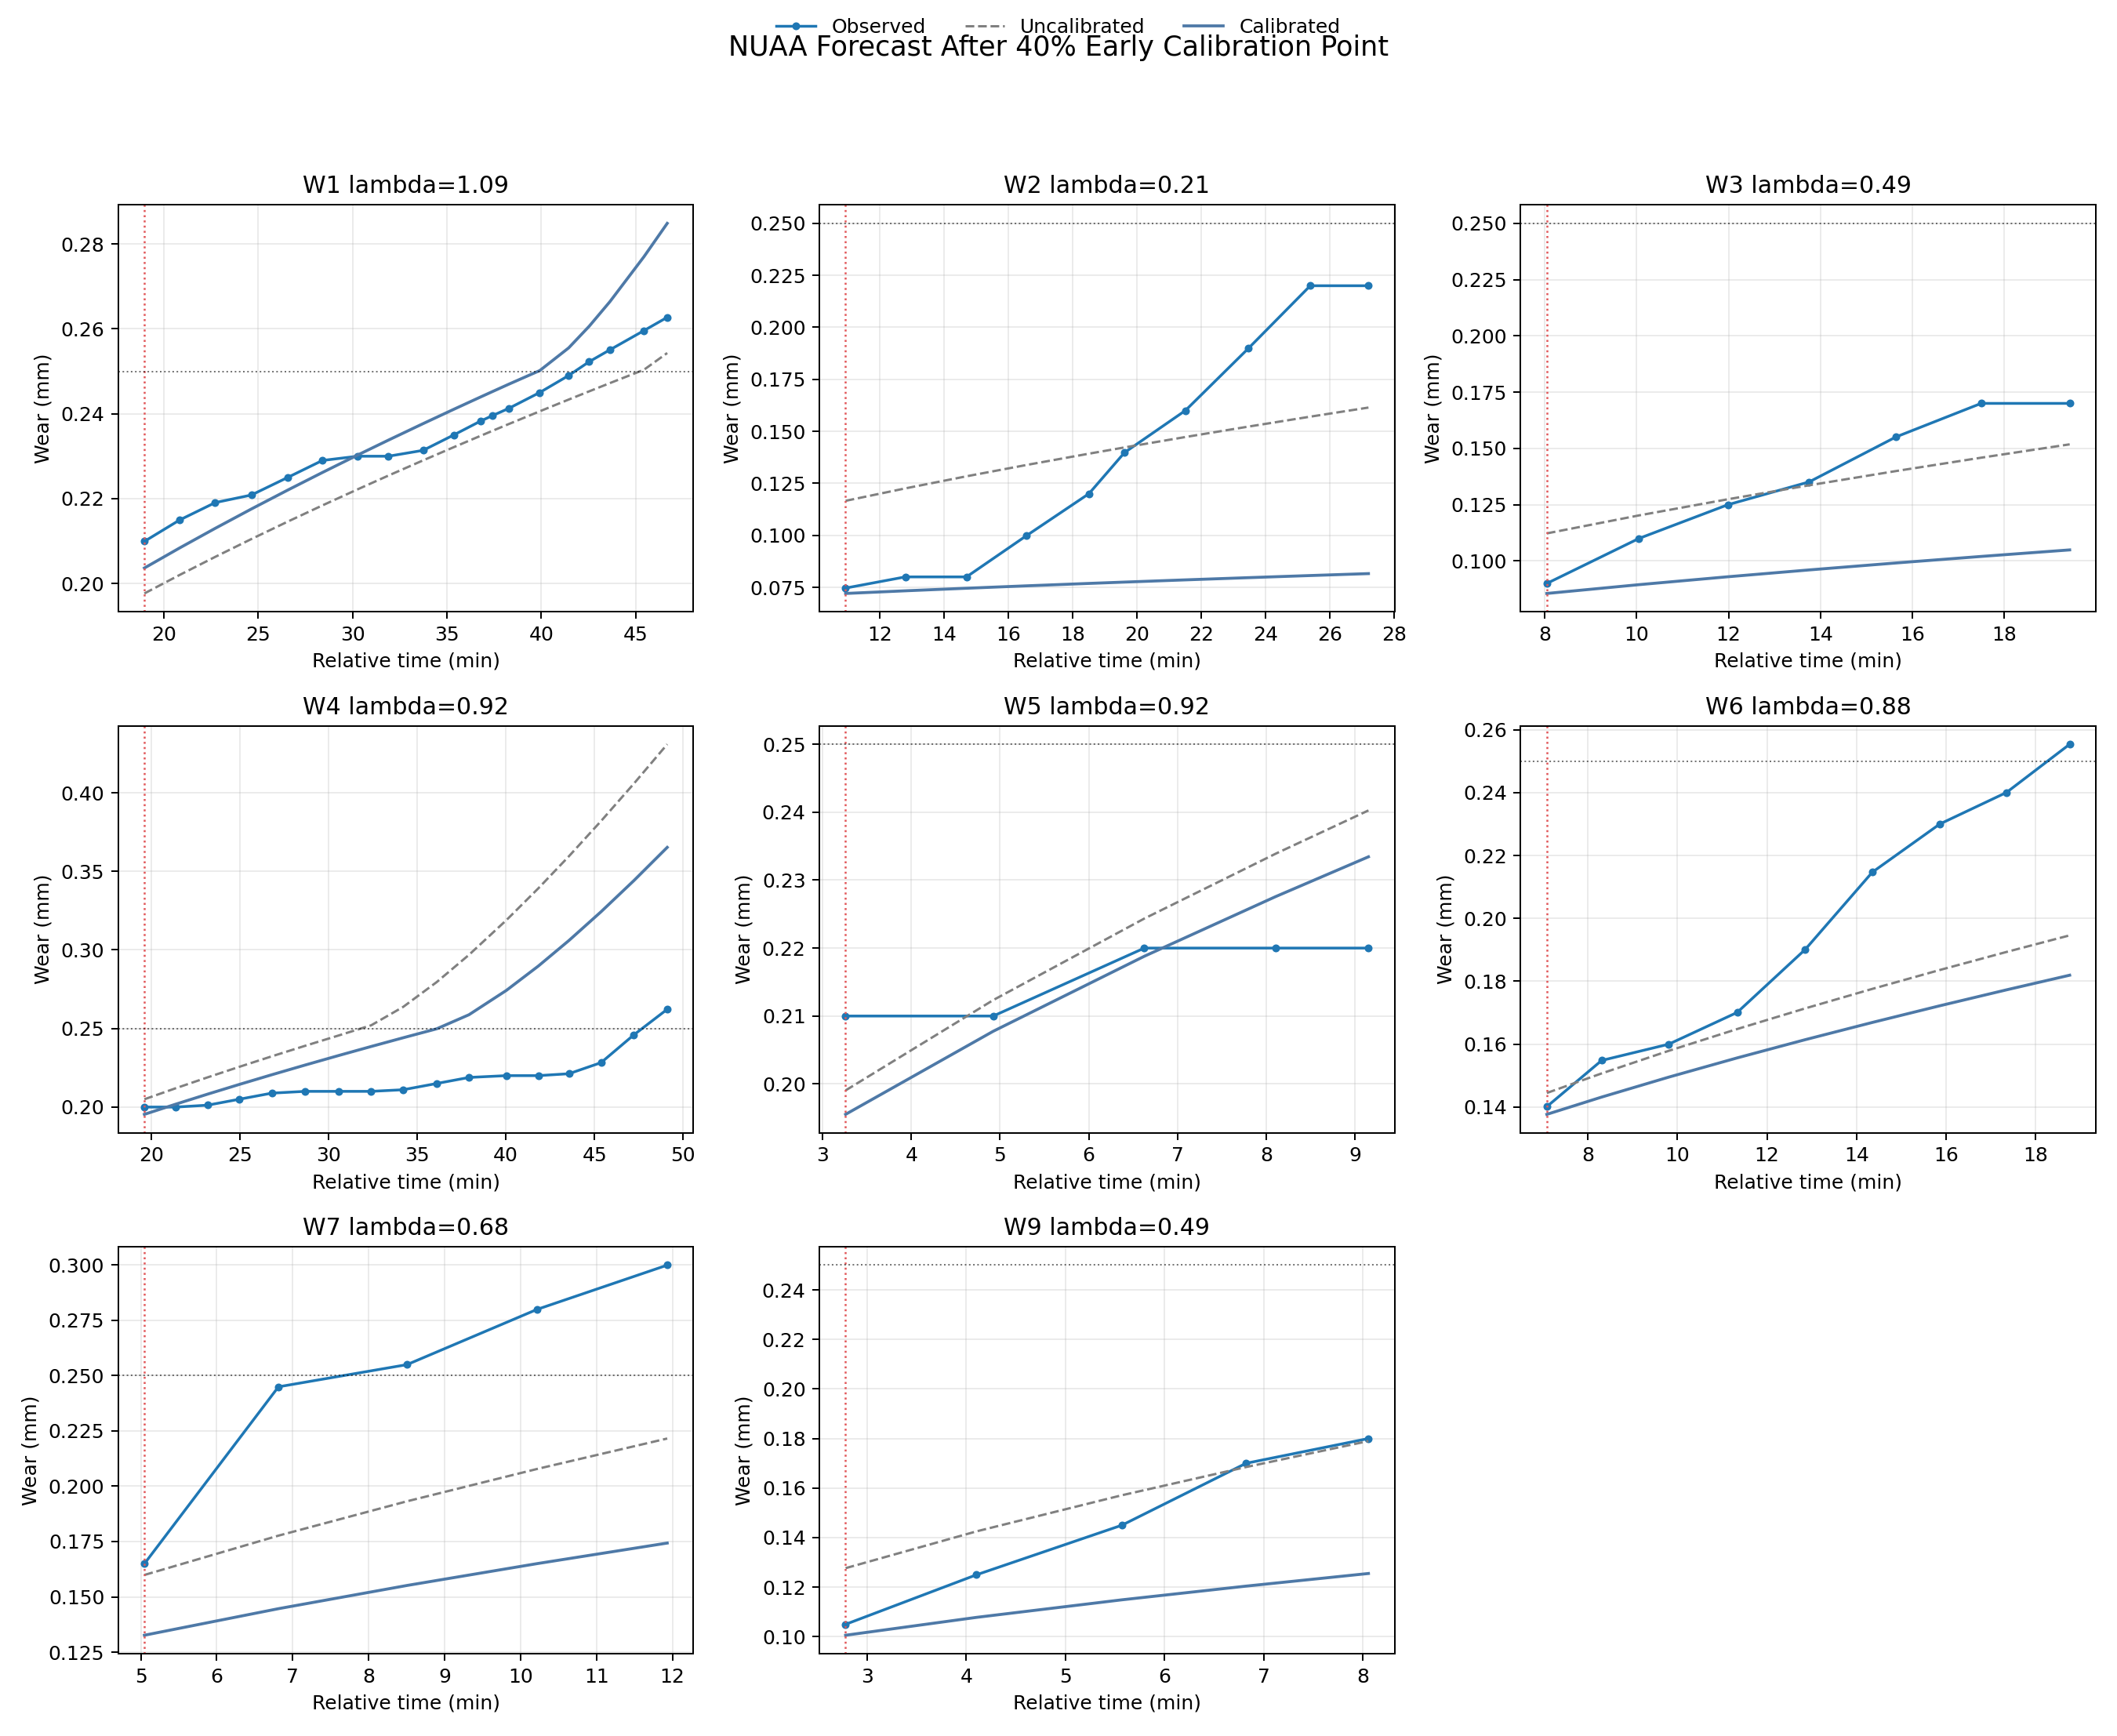
\includegraphics[width=0.78\textwidth]{nuaa_calibration_forecast.png}
  \caption{Calibration forecast diagnostic. Short-window calibration can overcorrect and worsen holdout forecasts in the local NUAA experiment set.}
  \label{fig:nuaa-calibration}
\end{figure}

\subsubsection{Residual Diagnostics}

Residual diagnostics show that the piecewise equation is most accurate in PHM2010 and NUAA early regimes, and least accurate in NASA, where severe wear, material variation, and late-stage behavior are stronger.

\begin{table}[!htbp]
  \centering
  \caption{Residual diagnostics for the Phase 2 equation.}
  \label{tab:residual-diagnostics}
  \small
  \begin{tabular}{lrrrrr}
    \toprule
    Dataset & Points & Bias & MAE & RMSE & 95\% abs. error \\
    \midrule
    NASA & 146 & 0.00763 & 0.03149 & 0.04376 & 0.08825 \\
    NUAA & 152 & -0.00162 & 0.01568 & 0.02113 & 0.04087 \\
    PHM2010 & 945 & 0.00104 & 0.01070 & 0.01362 & 0.02437 \\
    \bottomrule
  \end{tabular}
\end{table}

\begin{figure}[!htbp]
  \centering
  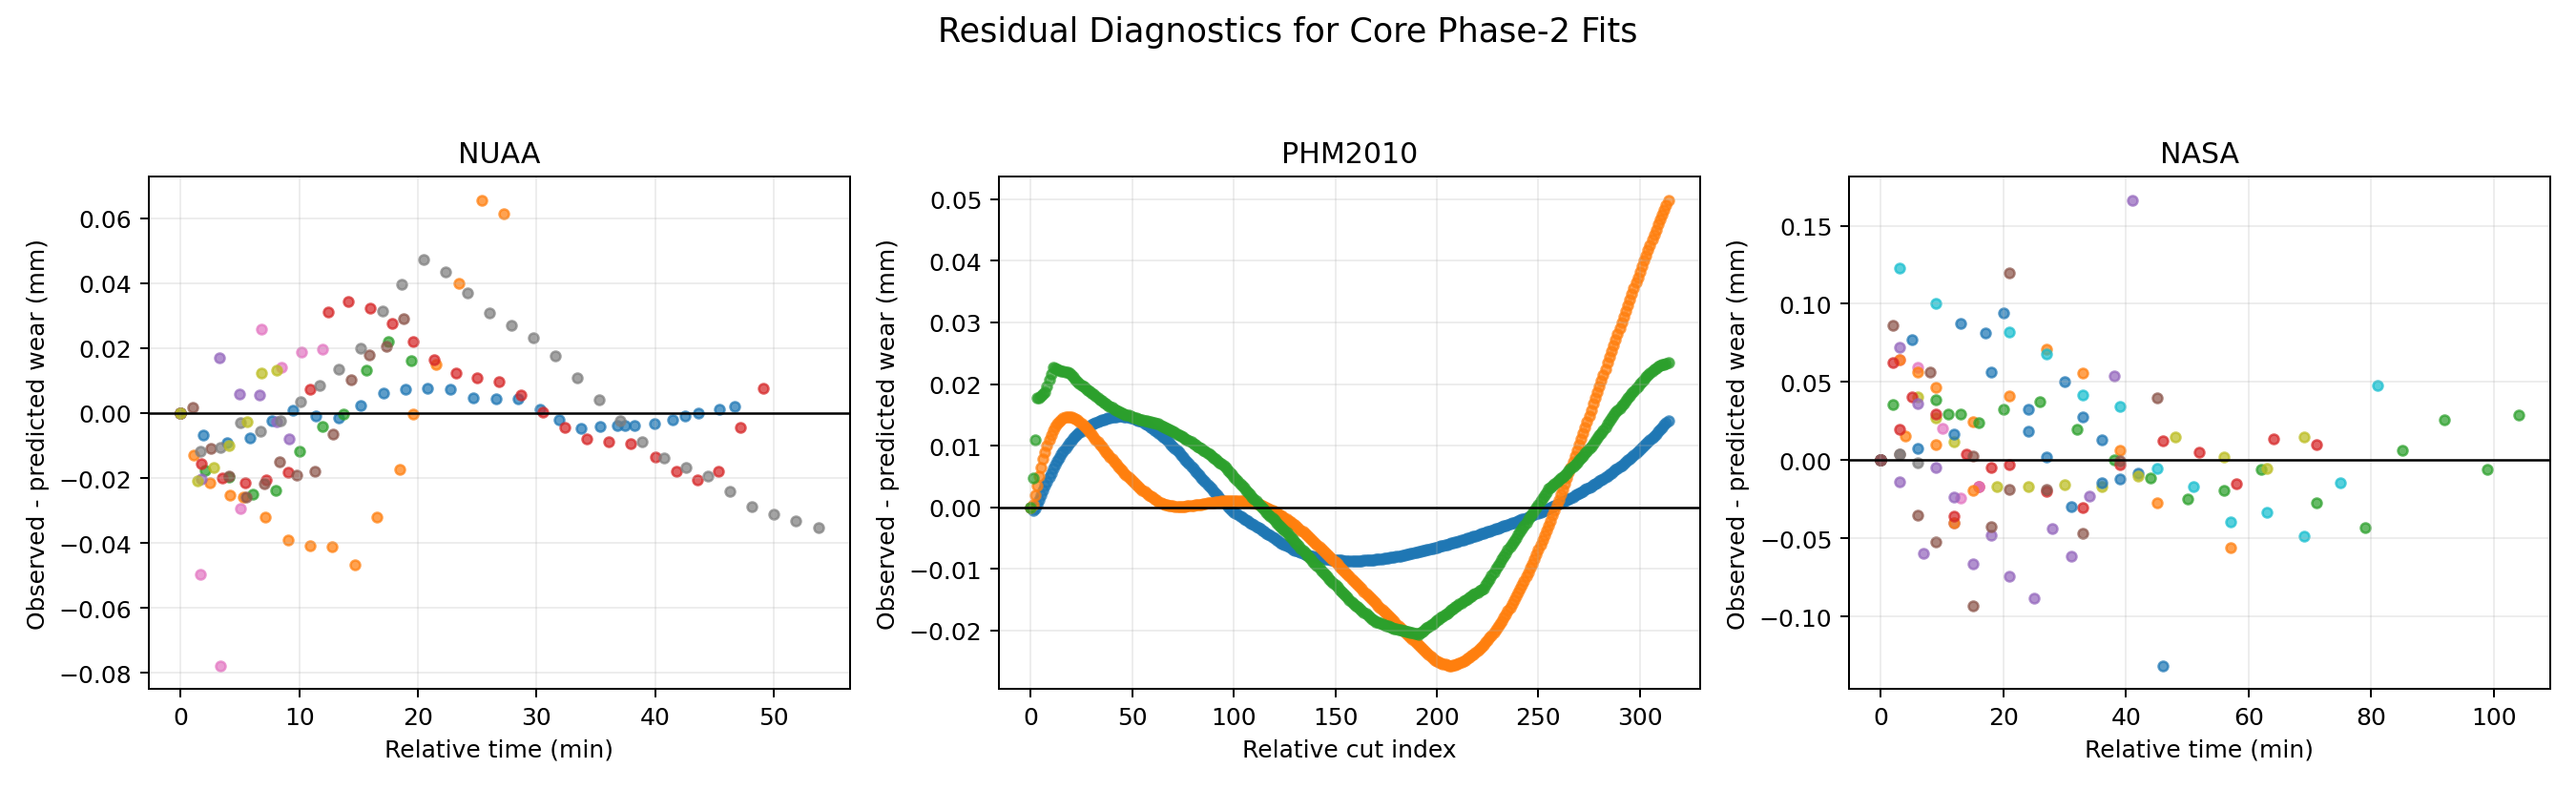
\includegraphics[width=0.82\textwidth]{residual_diagnostics.png}
  \caption{Residual diagnostics across datasets. The NASA tail remains the hardest local regime.}
  \label{fig:residual-diagnostics}
\end{figure}

\subsection{Lifetime Modeling by Training and Inverting Models}

\subsubsection{Why Wear Accuracy Is Not Enough}

The lifetime rework directly addressed whether tool life was estimated by training models and extracting results from those models. The answer is yes: NUAA wear models were trained, evaluated under leave-one-experiment-out validation, and inverted to estimate threshold-crossing life. The inversion step changes the target. A model can have low pointwise wear RMSE and still predict a poor crossing time if it is biased near the threshold.

\begin{figure}[!htbp]
  \centering
  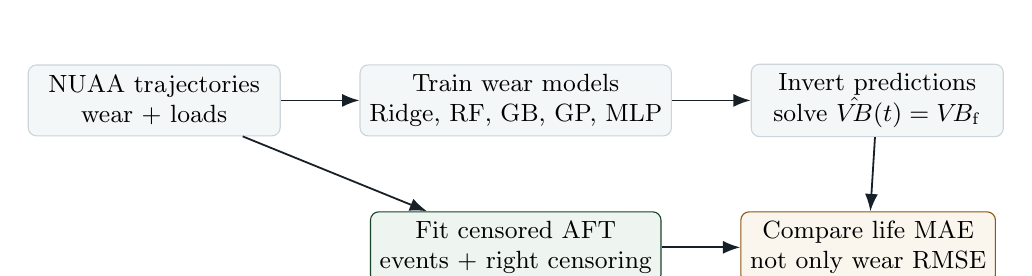
\begin{tikzpicture}[node distance=0.95cm and 1.0cm]
    \tikzset{
      block/.style={rounded corners=3pt,draw=linegray,fill=panel,minimum width=3.2cm,minimum height=0.9cm,align=center,font=\small},
      good/.style={rounded corners=3pt,draw=green!55!black,fill=green!8,minimum width=3.2cm,minimum height=0.9cm,align=center,font=\small},
      warn/.style={rounded corners=3pt,draw=amber!70!black,fill=amber!8,minimum width=3.2cm,minimum height=0.9cm,align=center,font=\small},
      arrow/.style={-{Latex[length=2.2mm]},draw=ink,line width=0.65pt}
    }
    \node[block] (data) {NUAA trajectories\\wear + loads};
    \node[block,right=of data] (train) {Train wear models\\Ridge, RF, GB, GP, MLP};
    \node[block,right=of train] (invert) {Invert predictions\\solve \(\hat{\vb}(t)=\vbf\)};
    \node[good,below=of train] (aft) {Fit censored AFT\\events + right censoring};
    \node[warn,right=of aft] (select) {Compare life MAE\\not only wear RMSE};
    \draw[arrow] (data) -- (train);
    \draw[arrow] (train) -- (invert);
    \draw[arrow] (data) -- (aft);
    \draw[arrow] (invert) -- (select);
    \draw[arrow] (aft) -- (select);
  \end{tikzpicture}
  \caption{Lifetime extraction workflow. The repository trains wear models, inverts them into crossing times, and compares them with survival-style equations.}
  \label{fig:lifetime-workflow}
\end{figure}

\subsubsection{Threshold-Crossing Labels}

Life labels were built by finding when each run crossed a dataset-specific wear threshold. Uncrossed runs were treated as censored. The time units were not mixed: NUAA and NASA lives are in minutes, while PHM2010 uses cutter cut index because its native time base differs.

\begin{table}[!htbp]
  \centering
  \caption{Threshold-crossing life labels.}
  \label{tab:life-labels}
  \small
  \begin{tabular}{lrrrr}
    \toprule
    Dataset & Records & Threshold & Events & Censored \\
    \midrule
    NUAA & 9 & 0.250 mm & 5 & 4 \\
    NASA & 15 & 0.300 mm & 15 & 0 \\
    PHM2010 & 3 & 0.150 mm & 3 & 0 \\
    \bottomrule
  \end{tabular}
\end{table}

\subsubsection{Trained Wear Models and Inverted Life}

\begin{table}[!htbp]
  \centering
  \caption{NUAA trained wear models and inverted event-life performance.}
  \label{tab:wear-life-benchmark}
  \small
  \begin{tabular}{lrrrrr}
    \toprule
    Model & Wear RMSE & Wear MAE & Wear \(R^2\) & Event-life MAE & Censor bound rate \\
    \midrule
    Phase2Equation & 0.0969 & 0.0460 & -0.8811 & 5.3832 & 1.00 \\
    Ridge & 0.0505 & 0.0407 & 0.4883 & 6.7010 & 0.75 \\
    Random Forest & 0.0457 & 0.0337 & 0.5817 & 8.9847 & 1.00 \\
    Gradient Boosting & 0.0394 & 0.0310 & 0.6896 & 11.6555 & 1.00 \\
    Gaussian Process & 0.0607 & 0.0459 & 0.2631 & 16.1923 & 1.00 \\
    MLP & 0.1159 & 0.0956 & -1.6890 & 19.0334 & 0.50 \\
    \bottomrule
  \end{tabular}
\end{table}

The best pointwise wear model is \textbf{Gradient Boosting}, but its event-life MAE is \emph{worse} than the Phase 2 equation and Ridge. This is a \textbf{strong negative result}: the lifetime problem cannot be judged only by \(\vb\) regression error. The selected model for extracting an interpretable life surface is \textbf{Ridge} because it is smoother and more reliable for inversion, even though it is not the lowest-RMSE wear model.

\begin{figure}[!htbp]
  \centering
  \begin{subfigure}{0.48\textwidth}
    \centering
    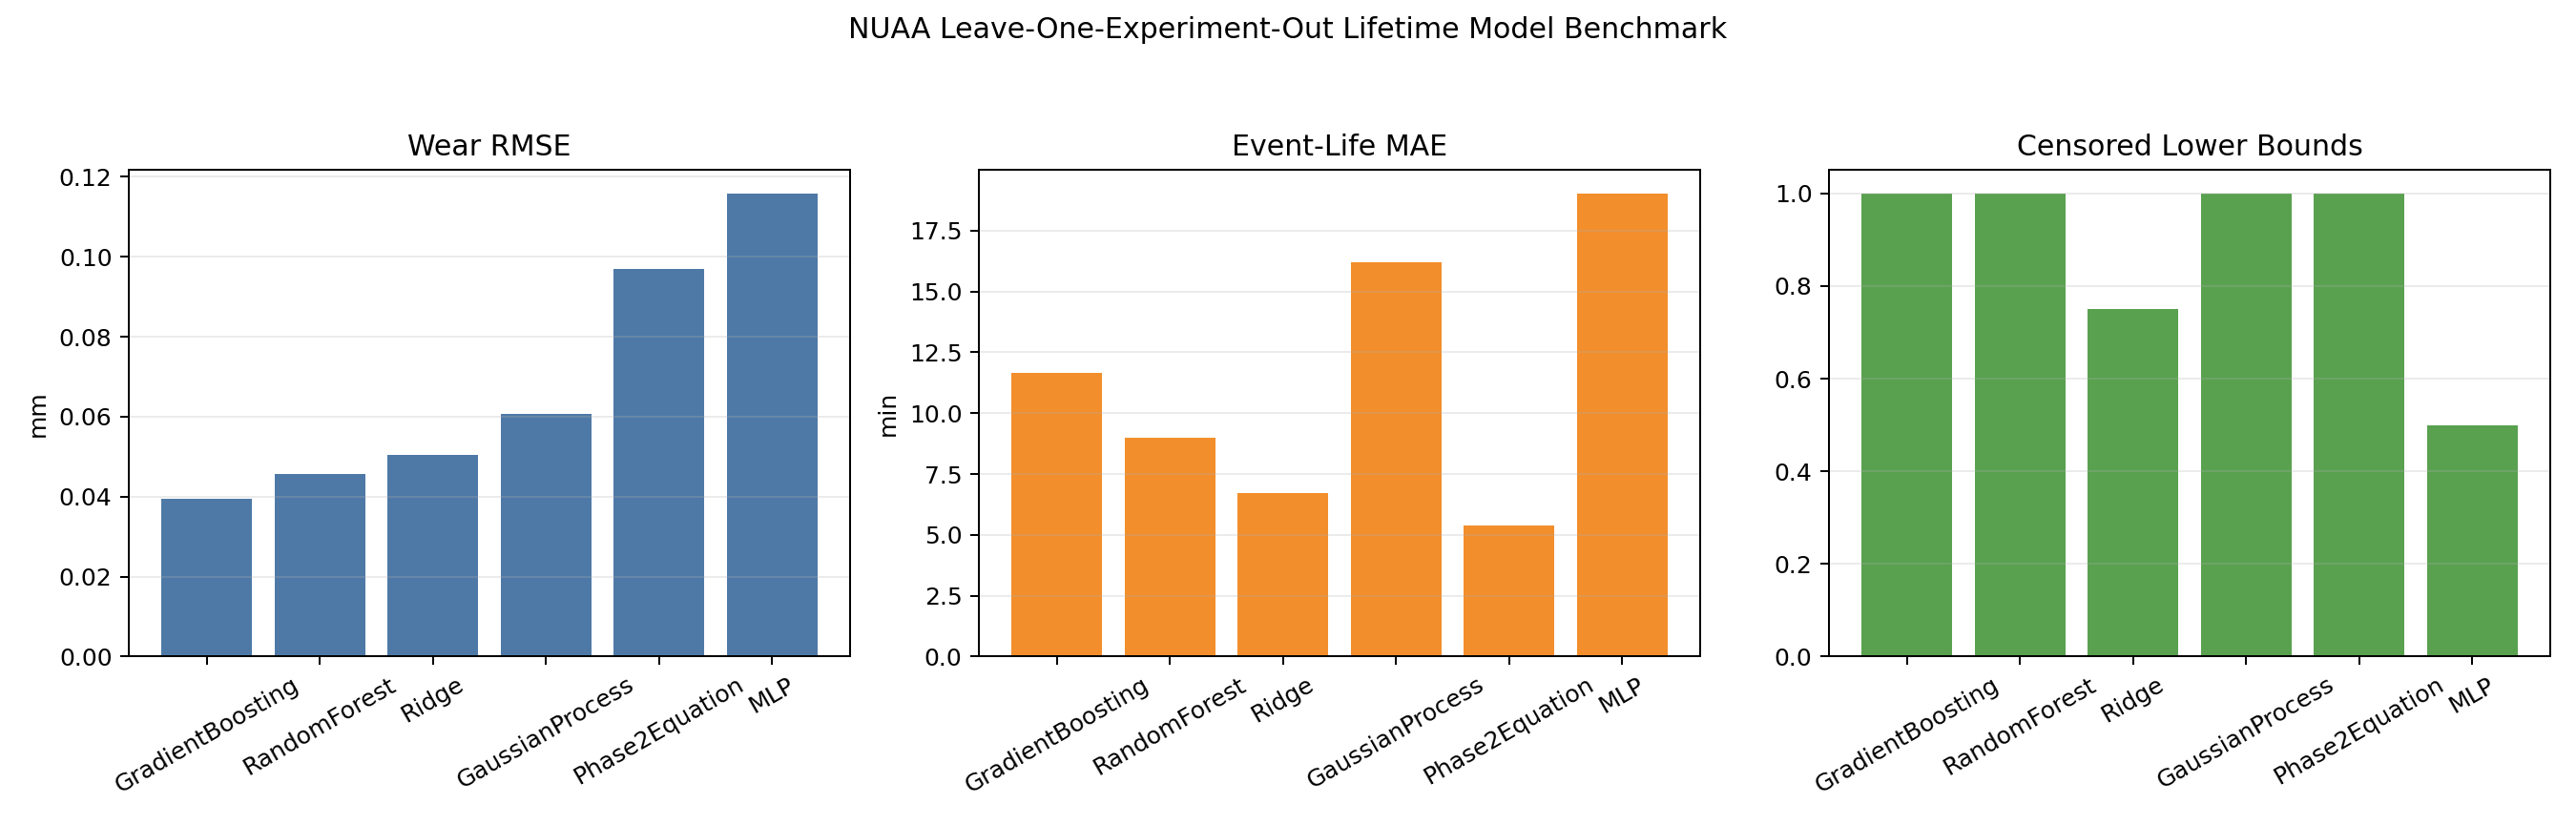
\includegraphics[width=\textwidth]{nuaa_wear_life_model_benchmark.png}
    \caption{Wear and life benchmark}
  \end{subfigure}
  \hfill
  \begin{subfigure}{0.48\textwidth}
    \centering
    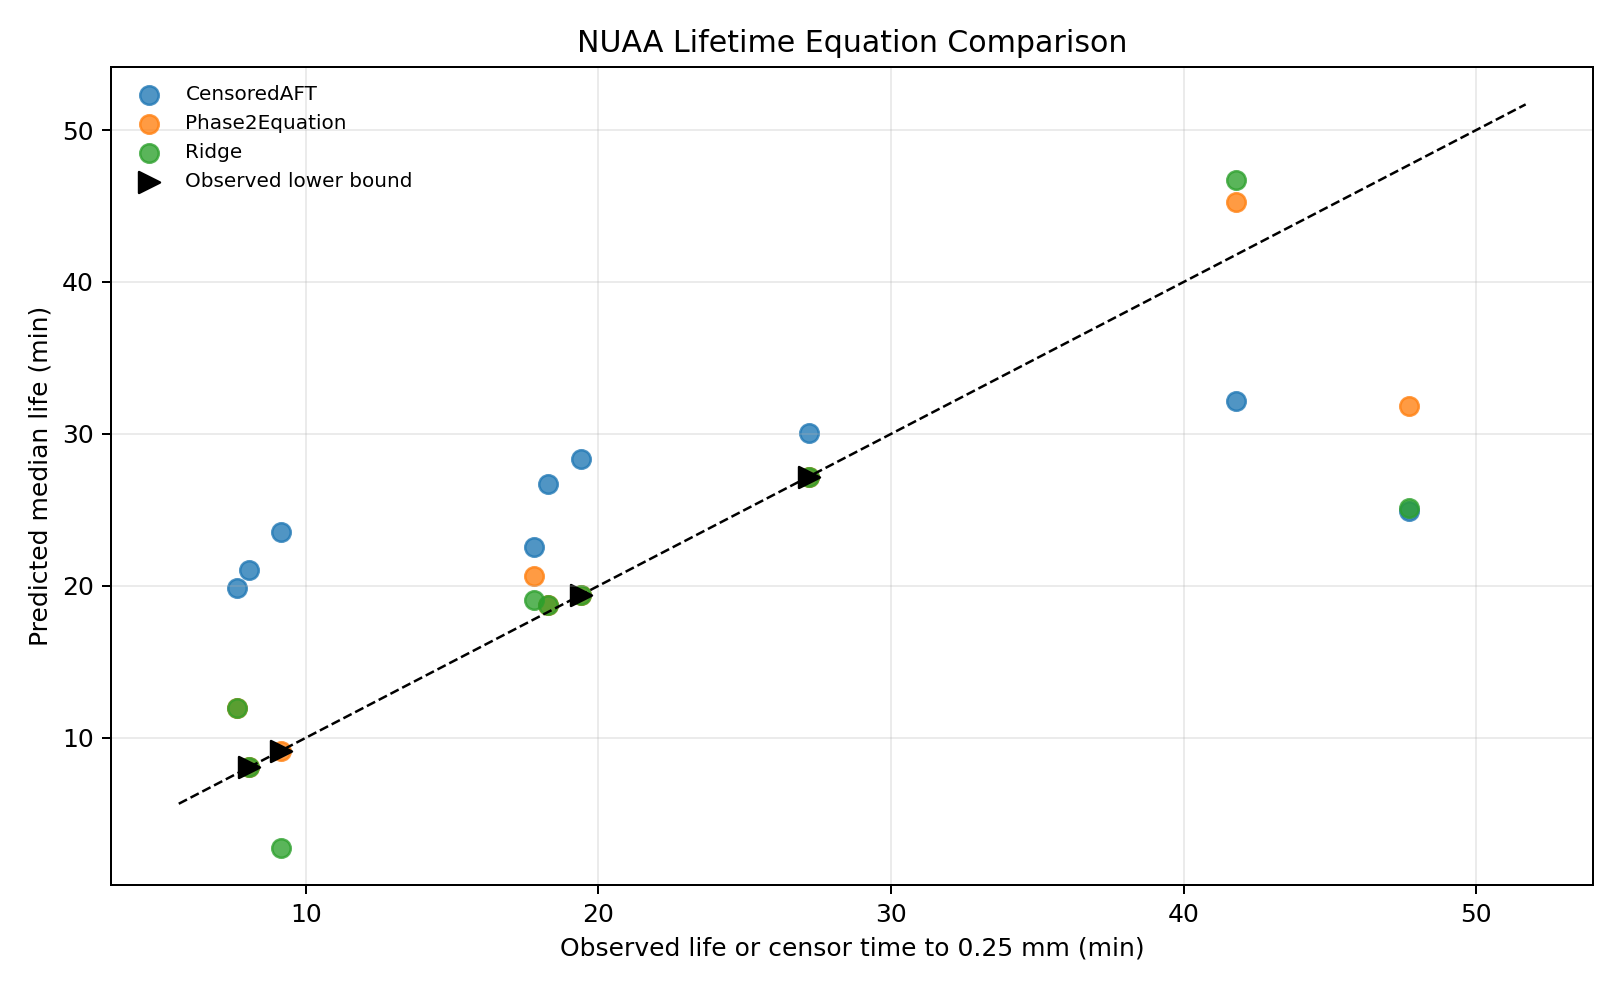
\includegraphics[width=\textwidth]{nuaa_life_equation_comparison.png}
    \caption{Life equation comparison}
  \end{subfigure}
  \caption{Wear-model inversion changes the model-selection problem. Smoothness near the threshold matters.}
  \label{fig:wear-life-benchmark}
\end{figure}

\subsubsection{Censored AFT Equation}

The NUAA censored accelerated-failure-time model is

\begin{equation}
T_{\min} =
24.93
\left(\frac{n}{1800}\right)^{-0.0187}
\left(\frac{f_z}{0.05}\right)^{-1.7662}
\left(\frac{a_p}{3.0}\right)^{-0.3768},
\label{eq:nuaa-aft}
\end{equation}

with \(\sigma=0.5291\) and negative log likelihood \(21.2365\). The AFT feed exponent is weaker than the Phase 2 condition-law feed exponent because it models sparse threshold-crossing events with censoring, not dense early wear amplitudes.

\begin{table}[!htbp]
  \centering
  \caption{NUAA AFT bootstrap coefficients.}
  \label{tab:aft-bootstrap}
  \small
  \begin{tabular}{lrrr}
    \toprule
    Coefficient & 2.5\% & Median & 97.5\% \\
    \midrule
    Intercept & 2.7199 & 3.2103 & 3.8286 \\
    log speed & -6.2471 & -0.2186 & 0.9129 \\
    log feed & -7.4945 & -2.1886 & 0.1153 \\
    log depth & -2.4450 & -0.5467 & 4.5558 \\
    sigma & 0.0000 & 0.1826 & 0.6821 \\
    \bottomrule
  \end{tabular}
\end{table}

\begin{figure}[!htbp]
  \centering
  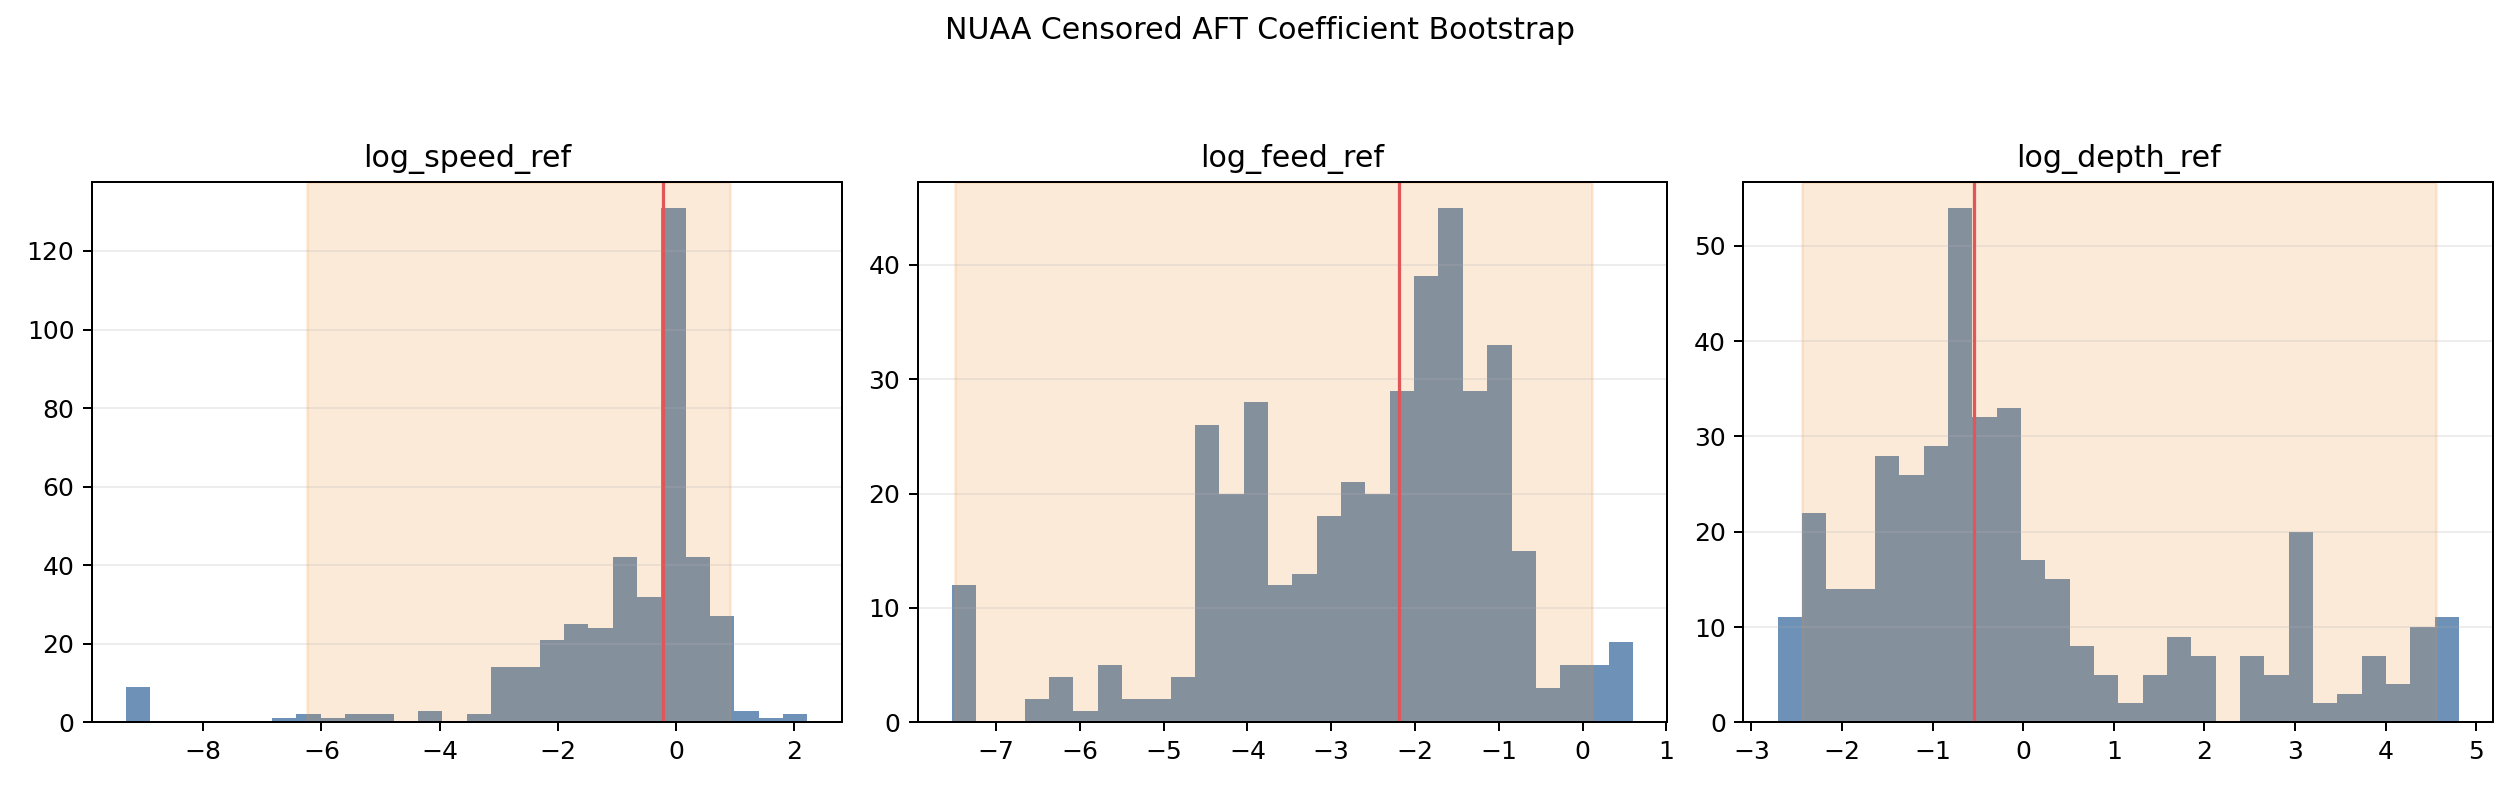
\includegraphics[width=0.78\textwidth]{nuaa_aft_coefficient_bootstrap.png}
  \caption{NUAA AFT bootstrap uncertainty. Sparse events and censoring make speed and depth effects weakly identified.}
  \label{fig:aft-bootstrap}
\end{figure}

\subsubsection{ML-Inverted Life Surface}

The Ridge response surface was inverted over a grid of operating scenarios and then compressed into a Taylor-like equation:

\begin{equation}
T_{\min} =
47.52
\left(\frac{n}{1800}\right)^{-10.4924}
\left(\frac{f_z}{0.05}\right)^{-4.6506}
\left(\frac{a_p}{3.0}\right)^{-0.1372},
\label{eq:ridge-life-surface}
\end{equation}

with surrogate log-space \(R^2=0.9800\) over 345 crossing scenarios. The high speed exponent should not be overinterpreted. It is a warning that the local speed range is narrow and speed is partly confounded with other load effects. The feed exponent is more consistent with the Phase 2 condition law and observed-life equation.

\begin{figure}[!htbp]
  \centering
  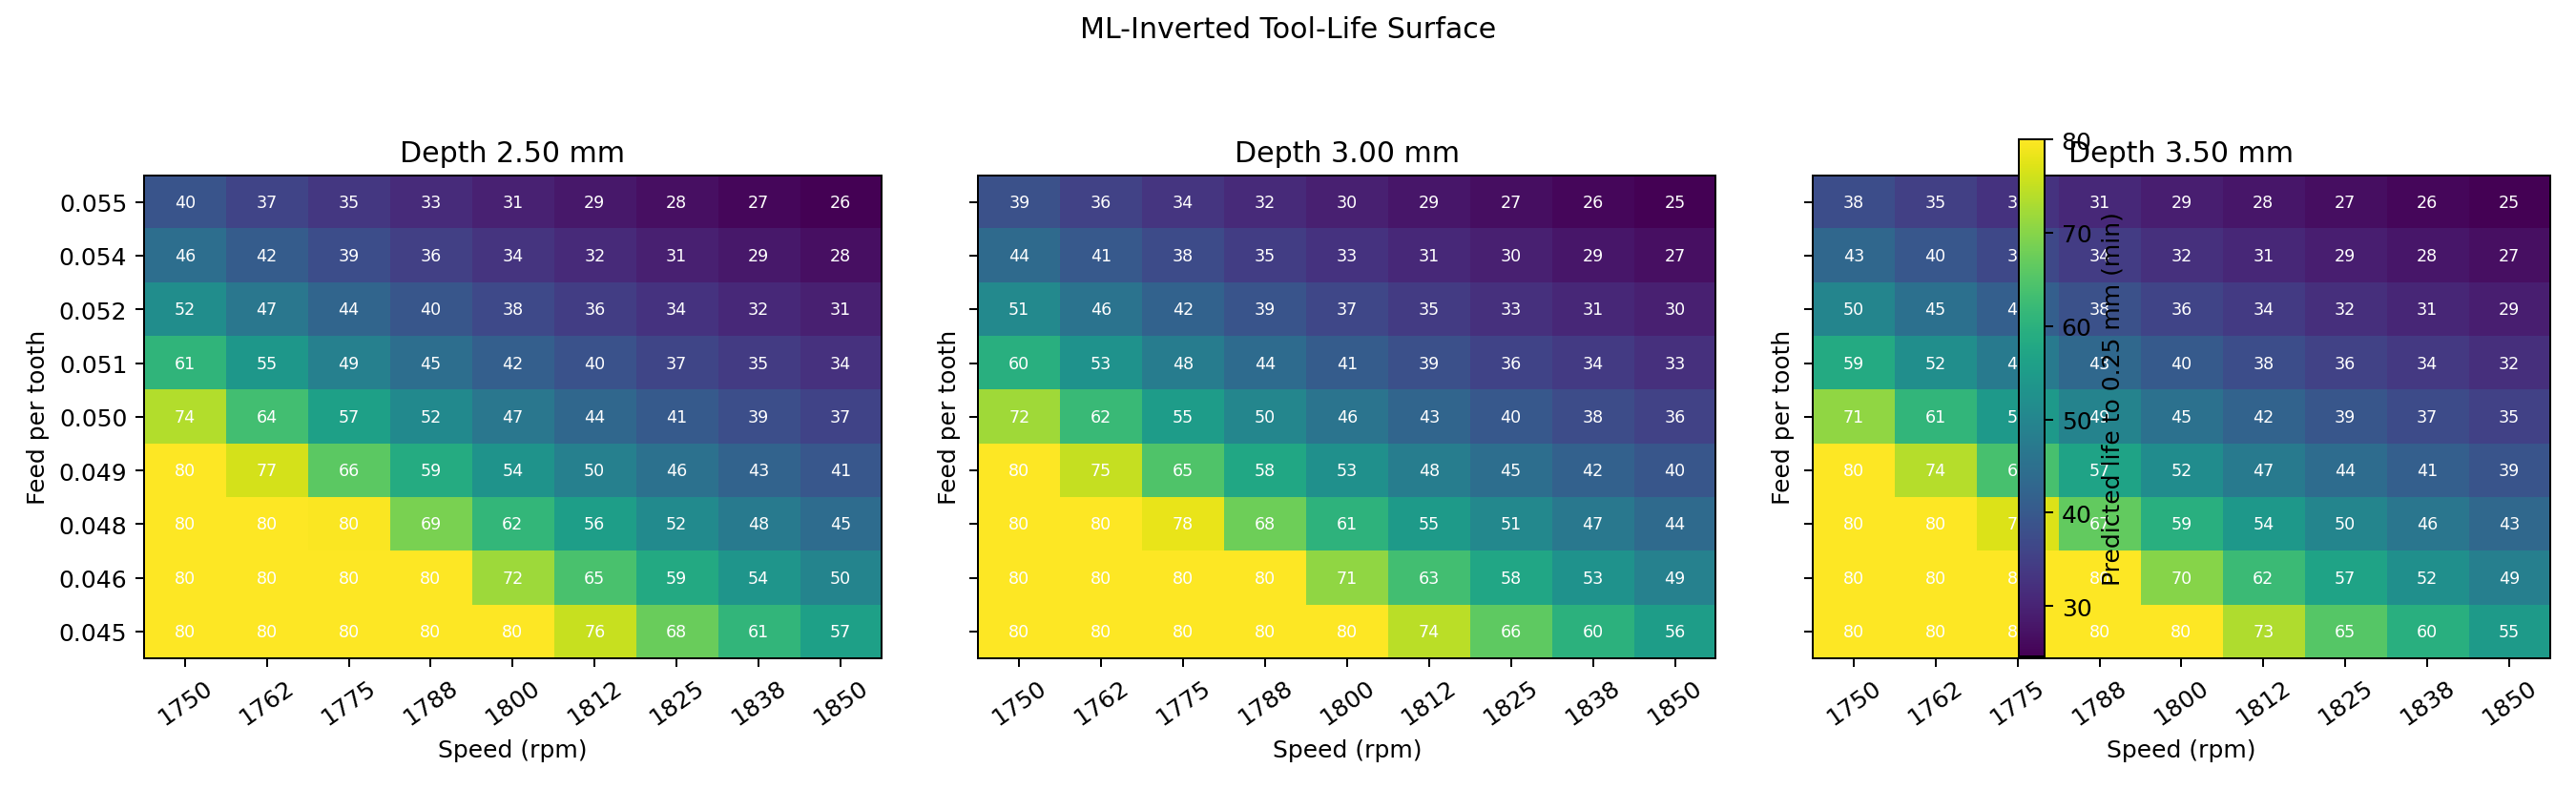
\includegraphics[width=0.8\textwidth]{ml_life_surface_heatmap.png}
  \caption{ML-inverted NUAA life surface. The surface is useful for scenario ranking but must be interpreted through the design limits of the training data.}
  \label{fig:ml-life-surface}
\end{figure}

\subsubsection{Direct Observed-Life Equation}

Using only uncensored NUAA threshold crossings yields

\begin{equation}
T_{\min} =
16.78
\left(\frac{n}{1800}\right)^{-12.6655}
\left(\frac{f_z}{0.05}\right)^{-4.1634}
\left(\frac{a_p}{3.0}\right)^{-2.4111},
\label{eq:observed-life}
\end{equation}

with log RMSE \(0.3784\). This equation is less robust because it discards censored runs. It is nevertheless useful as an independent check that feed has a strong negative effect on life.

\subsubsection{NASA Material-Aware AFT}

NASA is handled separately because its feed units, material families, fixed speed, and wear scale differ from NUAA. The material-aware AFT model includes feed, depth, material, and initial wear:

\begin{table}[!htbp]
  \centering
  \caption{NASA material-aware AFT model summary.}
  \label{tab:nasa-aft}
  \small
  \begin{tabular}{lrr}
    \toprule
    Term & Coefficient & Multiplicative effect \\
    \midrule
    Intercept & 4.0880 & 59.6220 \\
    log feed reference & -0.3874 & 0.6788 \\
    log depth reference & -1.1356 & 0.3212 \\
    material: steel & -1.6069 & 0.2005 \\
    initial wear & -3.1201 & 0.0442 \\
    \bottomrule
  \end{tabular}
\end{table}

The NASA AFT fit has event MAE \(2.5498\), RMSE \(3.1544\), \(R^2=0.9689\), \(\sigma=0.2459\), and negative log likelihood \(43.6327\). Because all NASA runs cross the threshold in this local label set, the model is not a censored survival problem in the same way as NUAA, but it provides strong evidence for material and initial-wear effects.

\begin{figure}[!htbp]
  \centering
  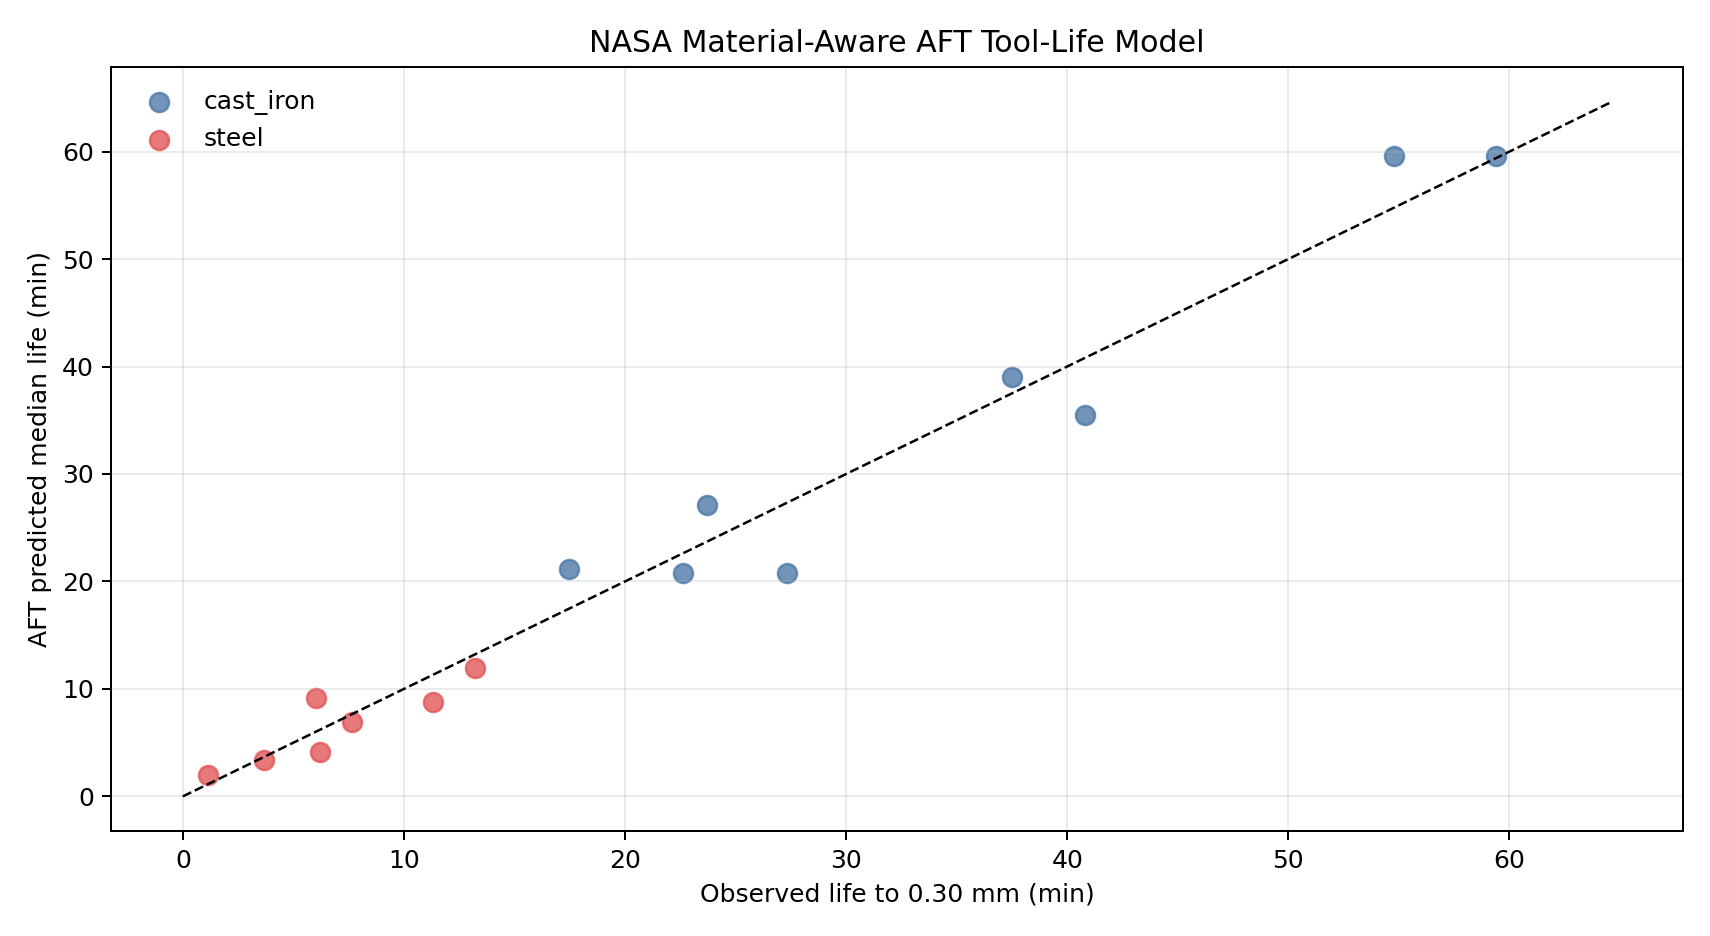
\includegraphics[width=0.78\textwidth]{nasa_aft_life_model.png}
  \caption{NASA material-aware AFT predictions. The high \(R^2\) is promising but should be interpreted with the small case count and fixed-speed design in mind.}
  \label{fig:nasa-aft}
\end{figure}

\subsection{Simulator and Digital-Twin Interpretation}

\subsubsection{From Equation to Simulator}

The repository includes a simulator-oriented Phase 2 model and frontend artifacts. The core simulator behavior is driven by the piecewise law and the load-intensity function. The simulator should be understood as a digital twin prototype: it maps operating conditions to wear trajectories and life estimates, but its uncertainty bands and known failure modes should remain visible.

\begin{figure}[!htbp]
  \centering
  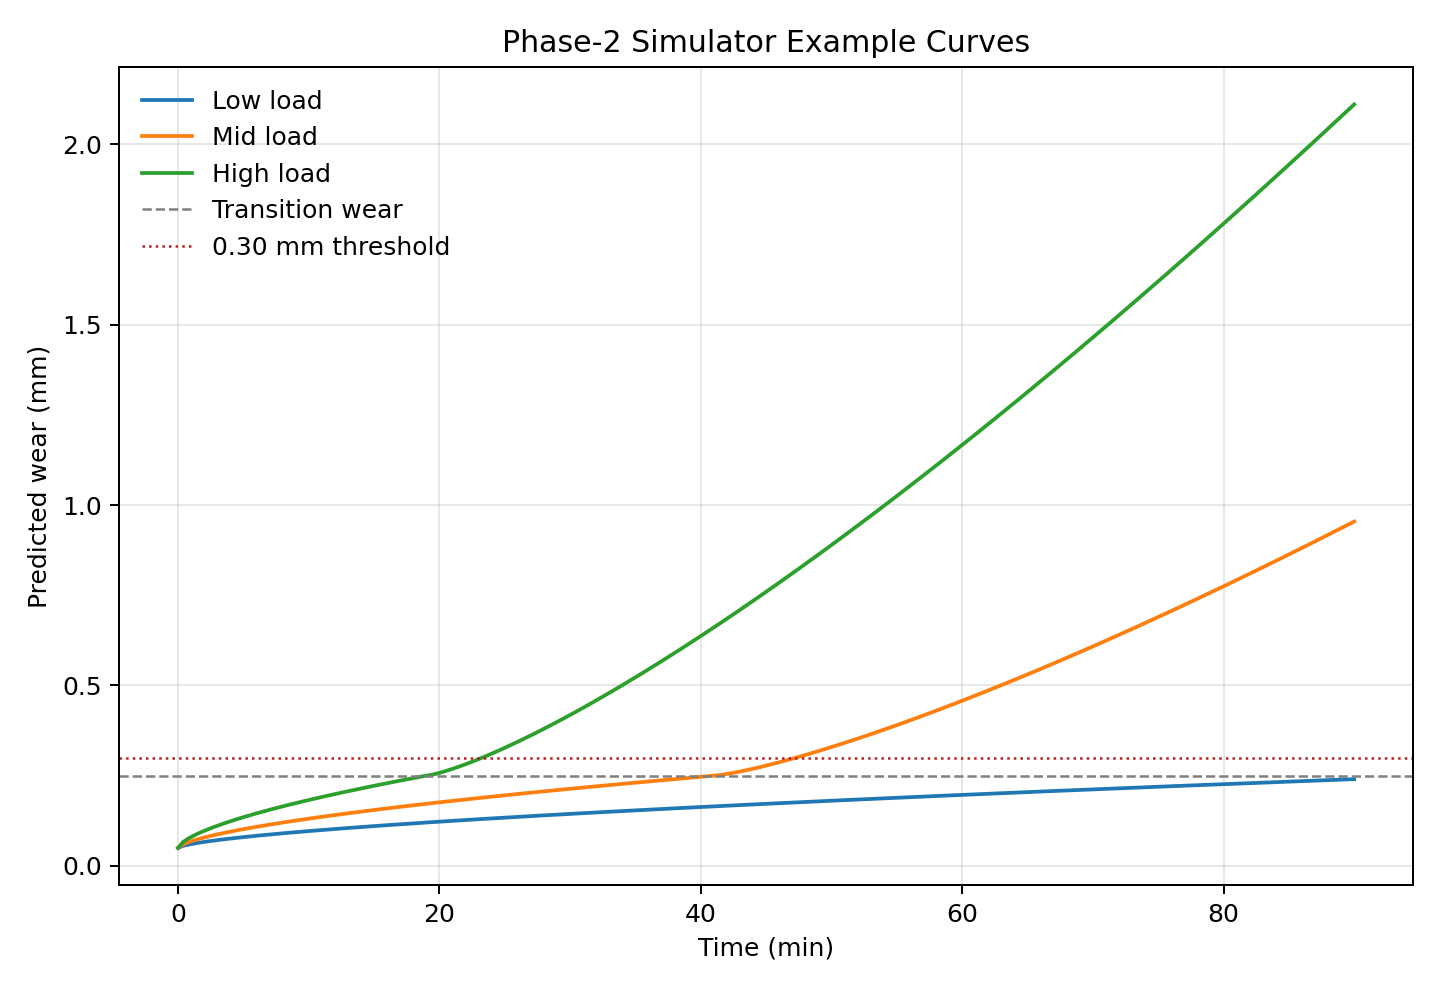
\includegraphics[width=0.78\textwidth]{simulation_example_curves.png}
  \caption{Example simulated wear curves. The piecewise law produces slow early growth followed by late acceleration.}
  \label{fig:simulation-curves}
\end{figure}

\subsubsection{Workload and Load-Effect Icons}

The operational story can be summarized with three load states. The icons below are intentionally simple LaTeX/TikZ marks rather than external artwork, so the document remains fully editable and portable.

\begin{figure}[!htbp]
  \centering
  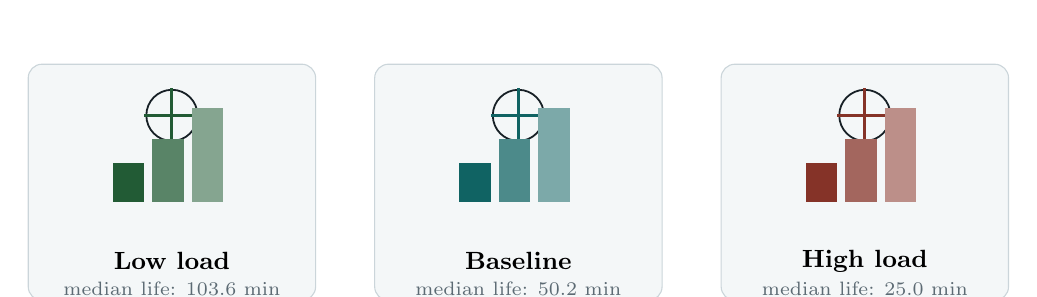
\begin{tikzpicture}[node distance=0.8cm]
    \tikzset{
      icon/.style={rounded corners=5pt,draw=linegray,fill=panel,minimum width=3.65cm,minimum height=3.0cm,align=center},
      gear/.style={circle,draw=ink,line width=0.65pt,minimum size=0.65cm},
      bar/.style={rounded corners=1pt,draw=none}
    }
    \node[icon] (low) at (0,0) {};
    \node[icon] (base) at (4.4,0) {};
    \node[icon] (high) at (8.8,0) {};
    \foreach \x/\c/\lab/\life in {0/green!75!black/Low load/103.6 min,4.4/teal!80!black/Baseline/50.2 min,8.8/brick!80!black/High load/25.0 min} {
      \node[gear] at (\x,0.85) {};
      \draw[\c,line width=1.1pt] (\x-0.35,0.85) -- (\x+0.35,0.85);
      \draw[\c,line width=1.1pt] (\x,0.5) -- (\x,1.2);
      \fill[\c] (\x-0.75,-0.25) rectangle (\x-0.35,0.25);
      \fill[\c!75] (\x-0.25,-0.25) rectangle (\x+0.15,0.55);
      \fill[\c!55] (\x+0.25,-0.25) rectangle (\x+0.65,0.95);
      \node[font=\small\bfseries] at (\x,-1.0) {\lab};
      \node[font=\scriptsize,color=muted] at (\x,-1.35) {median life: \life};
    }
  \end{tikzpicture}
  \caption{Load-effect icon comparison derived from bootstrap median life intervals. Higher feed/depth/speed compress predicted life.}
  \label{fig:load-icons}
\end{figure}

\subsubsection{Practical Decision Logic}

The current digital-twin logic should be used for scenario ranking and research exploration:

\begin{enumerate}
  \item Estimate the expected wear trajectory for a candidate load condition.
  \item Track sensor health markers, especially vibration and AE modal features, for deviation from the expected trajectory.
  \item Use survival-aware lifetime outputs when censoring or threshold crossing is the primary decision.
  \item Treat high-speed exponents and short-window calibrations carefully, because they are less stable in the local data.
\end{enumerate}

\begin{figure}[!htbp]
  \centering
  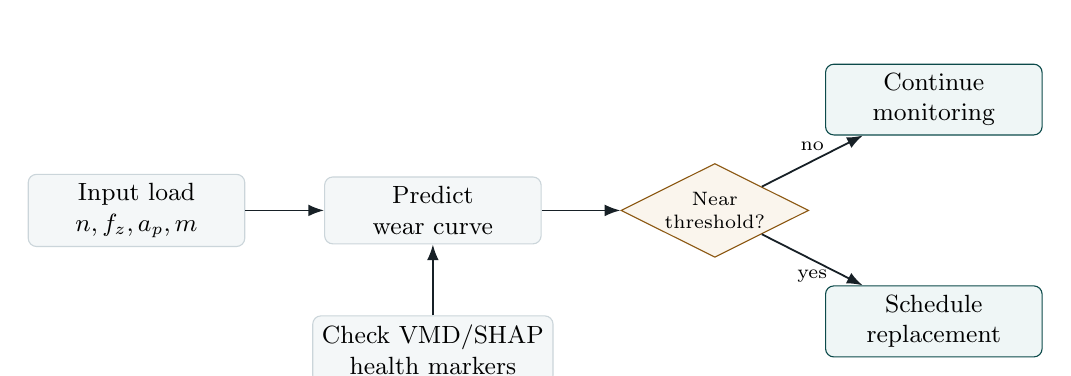
\begin{tikzpicture}[node distance=0.9cm and 1.0cm]
    \tikzset{
      flowstep/.style={rounded corners=3pt,draw=linegray,fill=panel,minimum width=2.75cm,minimum height=0.85cm,align=center,font=\small},
      decision/.style={diamond,aspect=2,draw=amber!70!black,fill=amber!8,align=center,font=\scriptsize,inner sep=1pt},
      action/.style={rounded corners=3pt,draw=teal!60!black,fill=teal!7,minimum width=2.75cm,minimum height=0.85cm,align=center,font=\small},
      arrow/.style={-{Latex[length=2mm]},draw=ink,line width=0.65pt}
    }
    \node[flowstep] (load) {Input load\\\(n,f_z,a_p,m\)};
    \node[flowstep,right=of load] (wear) {Predict\\wear curve};
    \node[decision,right=of wear] (thr) {Near\\threshold?};
    \node[action,above right=0.65cm and 0.8cm of thr] (continue) {Continue\\monitoring};
    \node[action,below right=0.65cm and 0.8cm of thr] (replace) {Schedule\\replacement};
    \node[flowstep,below=of wear] (signals) {Check VMD/SHAP\\health markers};
    \draw[arrow] (load) -- (wear);
    \draw[arrow] (wear) -- (thr);
    \draw[arrow] (thr) -- node[above,font=\scriptsize] {no} (continue);
    \draw[arrow] (thr) -- node[below,font=\scriptsize] {yes} (replace);
    \draw[arrow] (signals) -- (wear);
  \end{tikzpicture}
  \caption{Decision logic implied by the research. The simulator should combine physics-based wear trajectory estimates with sensor health markers.}
  \label{fig:decision-logic}
\end{figure}

\subsection{Limitations and Research Risk}

\subsubsection{Identified Limitations}

\begin{enumerate}
  \item The speed exponent is unstable in bootstrap and extracted life equations because the local speed range is narrow and correlated with other design variables.
  \item NASA provides strong late-stage and sensor evidence, but its feed units, material labels, and fixed-speed design make direct pooling with NUAA unsafe.
  \item PHM2010 is valuable for early-regime transfer, but the local use of PHM2010 has only three cutter groups.
  \item Gradient Boosting has the best NUAA pointwise wear RMSE but worse event-life MAE after threshold inversion, so model selection must follow the target decision.
  \item Per-run scalar calibration from short early windows overcorrects in NUAA holdout tests.
  \item The simulator is calibrated to the local datasets and should not be treated as an industrial replacement policy until validated on newer full-life milling datasets.
\end{enumerate}

\subsubsection{Risk Matrix}

\begin{table}[!htbp]
  \centering
  \caption{Research risk matrix.}
  \label{tab:risk-matrix}
  \small
  \begin{tabularx}{\textwidth}{p{3.0cm}p{2.0cm}p{2.0cm}Y}
    \toprule
    Risk & Severity & Current evidence & Recommended response \\
    \midrule
    Speed exponent overinterpretation & High & Wide bootstrap interval and large ML-inverted exponent & Report speed sensitivity as provisional and prioritize new experiments with wider speed variation. \\
    Dataset pooling mismatch & High & Different units, sensors, and thresholds & Maintain dataset-specific roles and use transfer learning only after unit harmonization. \\
    Calibration overcorrection & Medium & Calibrated RMSE worse than uncalibrated in NUAA & Replace scalar calibration with Bayesian or state-space updating. \\
    Small event count & High & NUAA has 5 events and 4 censored records & Add full-life datasets and keep censoring explicit. \\
    VMD feature overfitting & Medium & Many modal features relative to NASA sample count & Use grouped validation, feature stability, and sparse model variants. \\
    Simulator misuse & Medium & Simulator curves look decisive despite uncertainty & Surface intervals, limits, and dataset provenance in the UI. \\
    \bottomrule
  \end{tabularx}
\end{table}

\section{Conclusion}

\subsection{Recommended Next Experiments}

\subsubsection{Controlled Data Expansion}

The next research step is not to add more model classes first. It is to ingest broader full-life milling data under a strict provenance and validation plan. The 2025 QIT-CEMC and other open milling datasets listed in the research log are natural candidates. Each new dataset should be mapped into a common schema:

\begin{itemize}
  \item tool identifier, material, coating, cutter geometry, and workpiece material;
  \item cutting speed or spindle speed, feed per tooth or feed rate, axial/radial depth;
  \item wear measurement type, threshold definition, and native time base;
  \item available sensor channels, sampling rate, and preprocessing;
  \item event/censoring indicator at the chosen threshold.
\end{itemize}

\subsubsection{Modeling Roadmap}

\begin{figure}[!htbp]
  \centering
  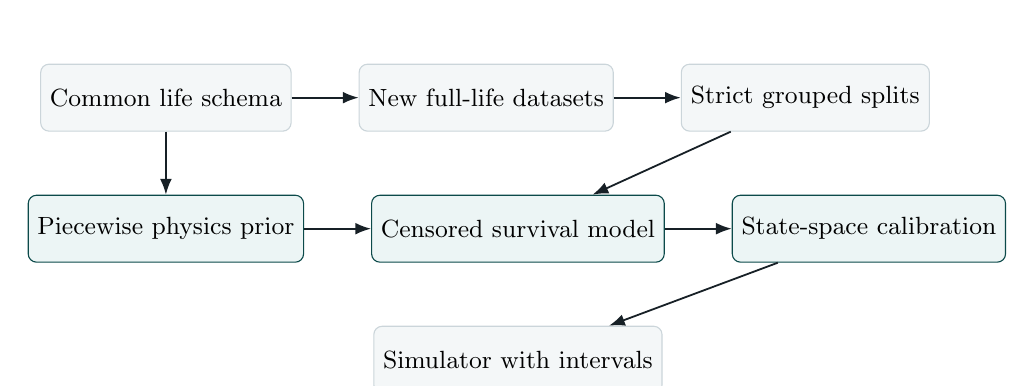
\begin{tikzpicture}[node distance=0.8cm and 0.85cm]
    \tikzset{
      item/.style={rounded corners=3pt,draw=linegray,fill=panel,minimum width=3.15cm,minimum height=0.85cm,align=center,font=\small},
      focus/.style={rounded corners=3pt,draw=teal!60!black,fill=teal!8,minimum width=3.15cm,minimum height=0.85cm,align=center,font=\small},
      arrow/.style={-{Latex[length=2mm]},draw=ink,line width=0.65pt}
    }
    \node[item] (schema) {Common life schema};
    \node[item,right=of schema] (ingest) {New full-life datasets};
    \node[item,right=of ingest] (split) {Strict grouped splits};
    \node[focus,below=of schema] (physics) {Piecewise physics prior};
    \node[focus,right=of physics] (survival) {Censored survival model};
    \node[focus,right=of survival] (state) {State-space calibration};
    \node[item,below=of survival] (ui) {Simulator with intervals};
    \draw[arrow] (schema) -- (ingest);
    \draw[arrow] (ingest) -- (split);
    \draw[arrow] (schema) -- (physics);
    \draw[arrow] (split) -- (survival);
    \draw[arrow] (physics) -- (survival);
    \draw[arrow] (survival) -- (state);
    \draw[arrow] (state) -- (ui);
  \end{tikzpicture}
  \caption{Recommended next modeling roadmap. The highest-value next work is structured dataset ingestion and survival-aware calibration, not simply adding more regressors.}
  \label{fig:roadmap}
\end{figure}

\subsubsection{Concrete Experiments}

\begin{enumerate}
  \item Refit the Phase 2 law after adding at least one full-life 2025 milling dataset.
  \item Run leave-dataset-out validation to measure whether the piecewise exponents transfer.
  \item Replace scalar calibration with a monotonic state-space update using sensor residuals.
  \item Train survival models that combine physics-law covariates with VMD feature summaries.
  \item Compare decision-level metrics: replacement lead time, missed-failure rate, false replacement rate, and expected unused tool life.
  \item Add uncertainty display to the simulator frontend so users see median and interval curves together.
\end{enumerate}

\subsection{Closing Remarks}

The repository now contains a coherent research program for milling tool wear and tool-life forecasting. The strongest technical result is \emph{not} a single machine-learning score; it is the combination of \textbf{interpretable physics, signal evidence, grouped validation, threshold inversion, and censoring-aware life modeling}. The piecewise wear law explains why early and late data should not be forced into one undifferentiated fit. The VMD and SHAP analyses show which sensor signatures carry wear information. The lifetime extraction pass shows that training a model and inverting it into life is possible, but also that \emph{the best wear regressor is not necessarily the best life predictor}.

The practical interpretation is clear. \textbf{Feed is the most reliable local load driver.} \textbf{Late-stage material behavior matters.} \textbf{Censoring must be modeled rather than ignored.} \textbf{Short-window scalar calibration is not yet dependable.} The current digital twin is ready for research simulation, scenario ranking, and explainer visualizations, but it needs larger full-life validation before industrial deployment.

\appendix

\section{Generated Artifact Index}

\footnotesize
\begin{longtable}{p{3.2cm}p{6.2cm}p{4.8cm}}
  \caption{Key local artifacts used in this monograph.}
  \label{tab:artifact-index}\\
  \toprule
  Artifact & Path & Purpose \\
  \midrule
  \endfirsthead
  \toprule
  Artifact & Path & Purpose \\
  \midrule
  \endhead
  Phase 2 summary & \path{phase -2/outputs/phase2_model_summary.json} & Core piecewise-law coefficients and plots. \\
  Extended report & \path{phase -2/outputs/extended_research/phase2_extended_research_report.md} & Bootstrap, intervals, calibration, residuals. \\
  Lifetime report & \path{phase -2/outputs/lifetime_modeling/phase2_lifetime_model_report.md} & Trained-model inversion and AFT results. \\
  Cross-dataset report & \path{results/cross_dataset_research/tool_health_failure_research_report.md} & Regression, classification, and failure marker results. \\
  VMD summary & \path{results/vmd/vmd_summary.txt} & Modal feature extraction and correlation summary. \\
  Interpretation summary & \path{results/interpretation/interpretation_summary.txt} & SHAP and ablation evidence. \\
  Research log & \path{phase -2/research_log.md} & Chronological record of extension and lifetime-modeling work. \\
  Sources log & \path{phase -2/sources.md} & Local and external source inventory. \\
  \bottomrule
\end{longtable}
\normalsize

\section{Equation Summary}

\begin{table}[!htbp]
  \centering
  \caption{Main equations produced by the research.}
  \label{tab:equation-summary}
  \small
  \begin{tabularx}{\textwidth}{p{3.1cm}Y}
    \toprule
    Model & Equation \\
    \midrule
    Condition intensity &
    \(\phii=(n/1800)^{0.359967}(f_z/0.05)^{3.956013}(a_p/3.0)^{0.688073}\) \\
    Early wear &
    \(\vb(t)=0.018580943\,\phii\,t^{0.64}\) \\
    NUAA censored AFT &
    \(T_{\min}=24.93(n/1800)^{-0.0187}(f_z/0.05)^{-1.7662}(a_p/3.0)^{-0.3768}\) \\
    Ridge-inverted life surface &
    \(T_{\min}=47.52(n/1800)^{-10.4924}(f_z/0.05)^{-4.6506}(a_p/3.0)^{-0.1372}\) \\
    Observed-life equation &
    \(T_{\min}=16.78(n/1800)^{-12.6655}(f_z/0.05)^{-4.1634}(a_p/3.0)^{-2.4111}\) \\
    NUAA Taylor-like observed lives &
    \(T\approx1.573{\times}10^{28}\,n^{-9.2806} f_z^{-4.6482} a_p^{-2.0471}\) \\
    \bottomrule
  \end{tabularx}
\end{table}

\renewcommand{\refname}{References}
\section*{References}
\addcontentsline{toc}{section}{References}

\begingroup
\setlength{\parindent}{0pt}
\setlength{\parskip}{0.4em}

Dragomiretskiy, K.\ and Zosso, D.\ (2014) `Variational mode decomposition', \emph{IEEE Transactions on Signal Processing}, 62(3), pp.~531--544.

Jain, A.K.\ and Lad, B.K.\ (2020) `Prognosticating RULs while exploiting the future characteristics of operating profiles', \emph{Reliability Engineering and System Safety}, 202, 107031.

Katzman, J.L., Shaham, U., Cloninger, A., Bates, J., Jiang, T.\ and Kluger, Y.\ (2018) `DeepSurv: personalized treatment recommender system using a Cox proportional hazards deep neural network', \emph{BMC Medical Research Methodology}, 18(1), 24.

Li, X., Lim, B.S., Zhou, J.H., Huang, S., Phua, S.J., Shaw, K.C.\ and Er, M.J.\ (2010) `Fuzzy neural network modelling for tool wear estimation in dry milling operation', in \emph{Proceedings of the Annual Conference of the Prognostics and Health Management Society} (PHM 2010 Data Challenge), San Diego, CA.

NASA Prognostics Center of Excellence (n.d.) \emph{Milling Data Set}. Available at: \url{https://www.nasa.gov/intelligent-systems-division/discovery-and-systems-health/pcoe/pcoe-data-set-repository/} (Accessed: April 2026).

Piecuch, G.\ and Zabinski, T.\ (2025) `Open milling tool-failure dataset and benchmark context', \emph{Scientific Data}, 12, pp.~1--14.

QIT-CEMC Consortium (2025) `QIT-CEMC: a full-life coated end-milling cutter wear dataset', \emph{Scientific Data}, 12, pp.~1--12.

Raissi, M., Perdikaris, P.\ and Karniadakis, G.E.\ (2019) `Physics-informed neural networks: a deep learning framework for solving forward and inverse problems involving nonlinear partial differential equations', \emph{Journal of Computational Physics}, 378, pp.~686--707.

Sankararaman, S.\ and Goebel, K.\ (2015) `Why is the remaining useful life prediction uncertain?', in \emph{Proceedings of the Annual Conference of the Prognostics and Health Management Society}, San Diego, CA, pp.~337--349.

Sun, H., Zhang, J., Mo, R.\ and Zhang, X.\ (2023) `In-process tool condition forecasting based on a deep learning method', \emph{Sensors}, 23(7), 3527.

UniWear / NUAA Consortium (n.d.) \emph{UniWear orthogonal milling wear records}. Nanjing University of Aeronautics and Astronautics. Local dataset documentation.

Wang, J., Xie, J., Zhao, R., Zhang, L.\ and Duan, L.\ (2017) `Multisensory fusion based virtual tool wear sensing for ubiquitous manufacturing', \emph{Robotics and Computer-Integrated Manufacturing}, 45, pp.~47--58.

Zhao, R., Yan, R., Chen, Z., Mao, K., Wang, P.\ and Gao, R.X.\ (2019) `Deep learning and its applications to machine health monitoring', \emph{Mechanical Systems and Signal Processing}, 115, pp.~213--237.

\endgroup

\end{document}
